\documentclass[11pt]{article}   	% use "amsart" instead of "article" for AMSLaTeX format
\usepackage[margin=1in]{geometry}
\geometry{letterpaper}
\usepackage[parfill]{parskip}    % Begins paragraphs with an empty line rather than an indent
\usepackage{graphicx}				% Use pdf, png, jpg, or eps§ with pdflatex; use eps in DVI mode
\usepackage{hyperref}			% Allows me to link in the text with \href{link}{description}
\usepackage{amssymb}
\usepackage{amsmath}
\usepackage{mathtools}
\usepackage{fancyhdr}
\usepackage{wrapfig}
\usepackage{xcolor}
\usepackage{titling}			% Allows me to set the \droptitle to make it less obnoxious
\usepackage{titlesec}			% Allows me to use \titlespacing command
\usepackage{blindtext}			% Allows me to generate Lorem Ipsum
\usepackage{pdfpages}			% Allows me to include pdf pages with the \includepdf[pages=-]{Filename.pdf} command
\renewcommand{\familydefault}{\sfdefault}	% uses san serif font
%\usepackage{cmss}			% changes font

% This was the order used for 
% Set text to 6 lines of 11pt font per 1 inch. Normal baseline skip is 13.6
% Source: https://tex.stackexchange.com/questions/23824/6-lines-in-one-inch
% 1 inch = 72.27pt
% First line is 11pts
% Remainder spread as (61.27/5)/13.6 = 0.901
%\linespread{0.901}

% Define useful shortcuts
\def\d{\text{d}}
\def\Pe{\text{Pe}}

% Spacing changes to make the document more compressed
\usepackage{enumitem}			% Allows me to set spacing to be more compressed for lists globally
\titlespacing{\section}{0em}{2em}{0em}		% Sauce: http://www.ctex.org/documents/packages/layout/titlesec.pdf, bottom p4
\setlist{nosep}								% Compresses all lists using enumitem package

% Headers
\pagestyle{fancy}
\lhead{Shannon Moran}

\title{Designing an information-driven pathway approach for targeted self-assembly}
\author{Shannon Moran}
\date{February 21, 2018}




\begin{document}

% =====
% TITLE PAGE
% =====
\maketitle
\thispagestyle{empty}
\noindent
This paper is submitted in partial fulfillment of the University of Michigan Chemical Engineering Department Preliminary Exam requirements.
\\ \\
\textbf{Committee:} 
\begin{quote} 
Prof. Sharon Glotzer (Advisor) \\ Prof. Ronald Larson \\ Prof. Robert Ziff \\ Prof. Xiaoming Mao (Cognate: Physics)
\end{quote}

% =====
% CONTENTS
% =====
\newpage
\thispagestyle{empty}


% =====
% ONE PAGE SUMMARY
% =====
%\newpage
%\thispagestyle{empty}
\section*{Project Summary: ``Designing an information-driven pathway approach for targeted self-assembly''}

% Include a self-contained description of the activity proposed;
% potential hazards and safety precautions should be identified;
% max one page

Self-assembly is a powerful tool for creating complex materials with tailored particle interactions.
Systems order with interactions as simple as hard-particle excluded volume and as complex as DNA-programmed origami. 
While much research has been focused on understanding how to design highly-specific building blocks and predict assembled structure, relatively little work has been focused on optimizing specificity in self-assembly system design.

Put another way-- 
\textbf{what is the minimal set of instructions needed to achieve targeted, self-assembled complexity?}

To investigate this question, we use a system of folding nets (of the five Platonic solids) with non-specific edge interactions.
Previous molecular dynamics studies of this system have shown that compact nets with more leaves are more likely to be able to fold into (i.e. assemble) the Platonic solid from which they were derived (i.e. their target structure).   
Authors observe that in these nets, folding pathways are enabled by the formation of local, native bonds, mirroring phenomena observed in protein folding.

This suggests that though the interactions are not specific, the combination of geometry and attraction serve to make some of these bonds more effective than others.
In turn, this suggests that it is possible to identify bonds that are more critical to assembly than others. 
If we are able to rank the importance of interactions on the yield of an assembly pathway, then it stands to reason that we can determine which interactions are the minimally sufficient set needed to guide assembly into a target structure. 

\textbf{Project 1: Define a measure of pathway information}\\
Studies have successfully developed measurements of the specificity (and resulting information capacity) for specific interactions of lock and key pairs.
However, no such metric exists linking a bond to the self-assembly yield of a starting configuration.
We propose developing a metric that measures the likelihood of a bond being a part of a successful assembly pathway-- i.e. the amount of mutual information between the bond and the final assembled structure.

Using this method, we can identify the most critical bonds for assembly and develop heuristics for identifying them in un-studied nets.
We can test our hypotheses that certain bonds are the most critical for successful assembly by incrementally adding bonds identified as ``critical'' to nets known to have poor yield of their target structure.
In this way, we can then also develop a measure of information efficiency of a structure relative to its target structure.
How much information must we give a system (in the form of specified bonds) for a starting material to reach its target structure at a given yield?

\textbf{Project 2: Develop energy landscapes for identifying kinetic barriers to assembly} \\
We hypothesize that seeding a structure with critical bonds can help a net avoid searching local minima en route to the global minimum. 
We can identify these local minima by building net disconnectivity graphs which convert a net's folding energy landscape into an easily-digestible network of free-energy minima and transition states.
Using these disconnectivity graphs, we will look for features of good- and poor-folding nets. 
Additionally, studying optimal energetic pathways may give us further insight into why nets with more leaves fold better than others.

\textbf{Project 3: Design pluripotent nets from minimal instructions} \\
Finally, understanding the minimum amount of instruction needed to drive a configuration to a given assembly opens the possibility of embedding instructions for multiple states into a starting material.
We call such a material pluripotent. 
Given the rules for minimal assembly instructions from Project 1 and the energy landscapes developed in Project 2, we will attempt to use a minimum set of specific bonds to embed multiple potential target structures into a net.



% =====
% MAIN TEXT
% =====
\clearpage
\setcounter{page}{1}


% =====
% MOTIVATION AND LITERATURE REVIEW
% =====
\section{Introduction}
% statement of problem
% purpose and significance

Self-assembly is a powerful tool for creating complex materials with tailored particle interactions.
Systems order with interactions as simple as hard-particle excluded volume \cite{Damasceno_2012_Science} and as complex as DNA-programmed origami \cite{Winfree_1998_Nature}. 
While much research has been focused on understanding how to design highly-specific building blocks and predict assembled structure, relatively little work has been focused on optimizing specificity in self-assembly system design.

Put another way-- 
\textbf{what is the minimal set of instructions needed to achieve targeted, self-assembled complexity?}

%To investigate this question, we use a system of folding nets (of the five Platonic solids) with non-specific edge interactions.
%Previous molecular dynamics studies of this system have shown that compact nets with more leaves are more likely to be able to fold into (i.e. assemble) the Platonic solid from which they were derived (i.e. their target structure).   
%Authors observe that in these nets, folding pathways are enabled by the formation of local, native bonds, mirroring phenomena observed in protein folding.
%
%This suggests that though the interactions are not specific, the combination of geometry and attraction serve to make some of these bonds more effective than others.
%In turn, this suggests that it is possible to identify bonds that are more critical to assembly than others. 
%If we are able to rank the importance of interactions on the yield of an assembly pathway, then it stands to reason that we can determine which interactions are the minimally sufficient set needed to guide assembly into a target structure. 

%Self-assembly is a powerful tool for creating materials by design.
%Systems of simple particles with programmed interactions are capable of creating a rich complexity of structures and behaviors.
%One of the key challenges of modern materials design is understanding self-assembly to use it to create even more complex structures.
%
%Here, we propose using a simple folding model of nets to develop methodology for identifying ``high information bonds''-- i.e., bonds that are critical to avoid kinetic traps and enabling further assembly.
%We propose using the methods and information metrics developed to then develop an ``information efficiency'', to determine the minimal amount of programmed interactions required to still reliably reach a target state.


%Colloidal-scale self-assembly is of particular interest. 
%Larger than atoms, colloids experience thermal fluctuations (and thus are well-characterized by statistical thermodynamics).
%Additionally, much research has been spent characterizing their behavior.
%They are easily synthesized in experiments, and can be simulated simply.

%Recent innovations in DNA-programmed assembly have demonstrated the ability to assemble specifically ordered arrangements of particles with both high complexity and high accuracy.
%The sequence-specific binding property of DNA can be applied to direct the assembly behavior of colloidal particles at the nanoscale.
%Theoretical work has shown that this powerful assembly shouldn't be limited to DNA systems, but rather accessible to any system with sufficiently specific interactions (including colloids) \cite{Reinhardt_2014_PRL}. 
%
%However, such highly-programmed assembly is prone to two problems.
%\begin{enumerate}
%\item Performance of assembly is highly reliant upon kinetics to avoid mis-matches or multiple nucleation events
%\item Exacting level of specificity required is currently only achievable with DNA methods
%\end{enumerate}

% could include something here about the relative citations on different papers-- there's something missing here; everything is too specific?

%Such an approach would provide a powerful toolkit for scientists looking to engineer colloidal systems with addressable complexity.

%\textbf{Key question: How can we \textit{most efficiently} direct a system to self-assemble?}


\section{Background}

% =====
% SELF-ASSEMBLY, GENERALLY
% =====

Self-assembly is the process by which individual components arrange themselves into an ordered structure via free energy minimization \cite{Whitesides_2002_Science}.
This ordered structure is determined by the inter-particle interactions and assembly environment, and much recent work has focused on tuning these parameters to achieve target structures \cite{Boles_2016_ChemRev}. 
With advances in material synthesis techniques, complex building blocks can now be made with nano- and micro-precision.
Correspondingly, there has been a focus in the literature to understand the role of building block properties on the bulk structure assembled.

At the colloidal scale, seemingly simple additions of anisotropic interactions to building blocks can yield complex structures \cite{GlotzerSolomon_2007_Nature}.
Hard particles with shape can assemble a rich variety of structures \cite{Damasceno_2012_Science}, even in the absence of explicit interactions between particles other than excluded volume.
Later work described this as the effect of an effective entropic patchiness caused by shape interactions \cite{vanAnders_2014_ACSNano}.

Even when specific interactions are added, they do not need to be complex for small changes to lead to very different structures.
Adding explicit attractive patches to otherwise isotropic particles led to the formation of shapes, clusters, and rings, depending on the orientation of the patches \cite{Zhang_2004_NanoLetters}.
Later, Millan \textit{et al.} were able to access Archimedean tilings of regular polygons by incrementally adding attraction to guide assembly to target structures \cite{Millan_2014_ACSNano}.
However, even non-specific directional attractive patches can cause particles (in one case, nanoplates forming a superlattice) to self-assemble structures differing from those accessible via entropic forces alone \cite{Ye_2013_NatChem}.
Experimentally, DNA-mediated particle interactions are now a powerful tool for tailoring crystal structure of a uniform building block \cite{Park_2008_Nature}.

The diversity of structures that can be accessed from simple interactions is impressive, and there is still much to be understood about how inter-particle interactions impact the structure assembled.

\begin{figure}[t]
\begin{center}
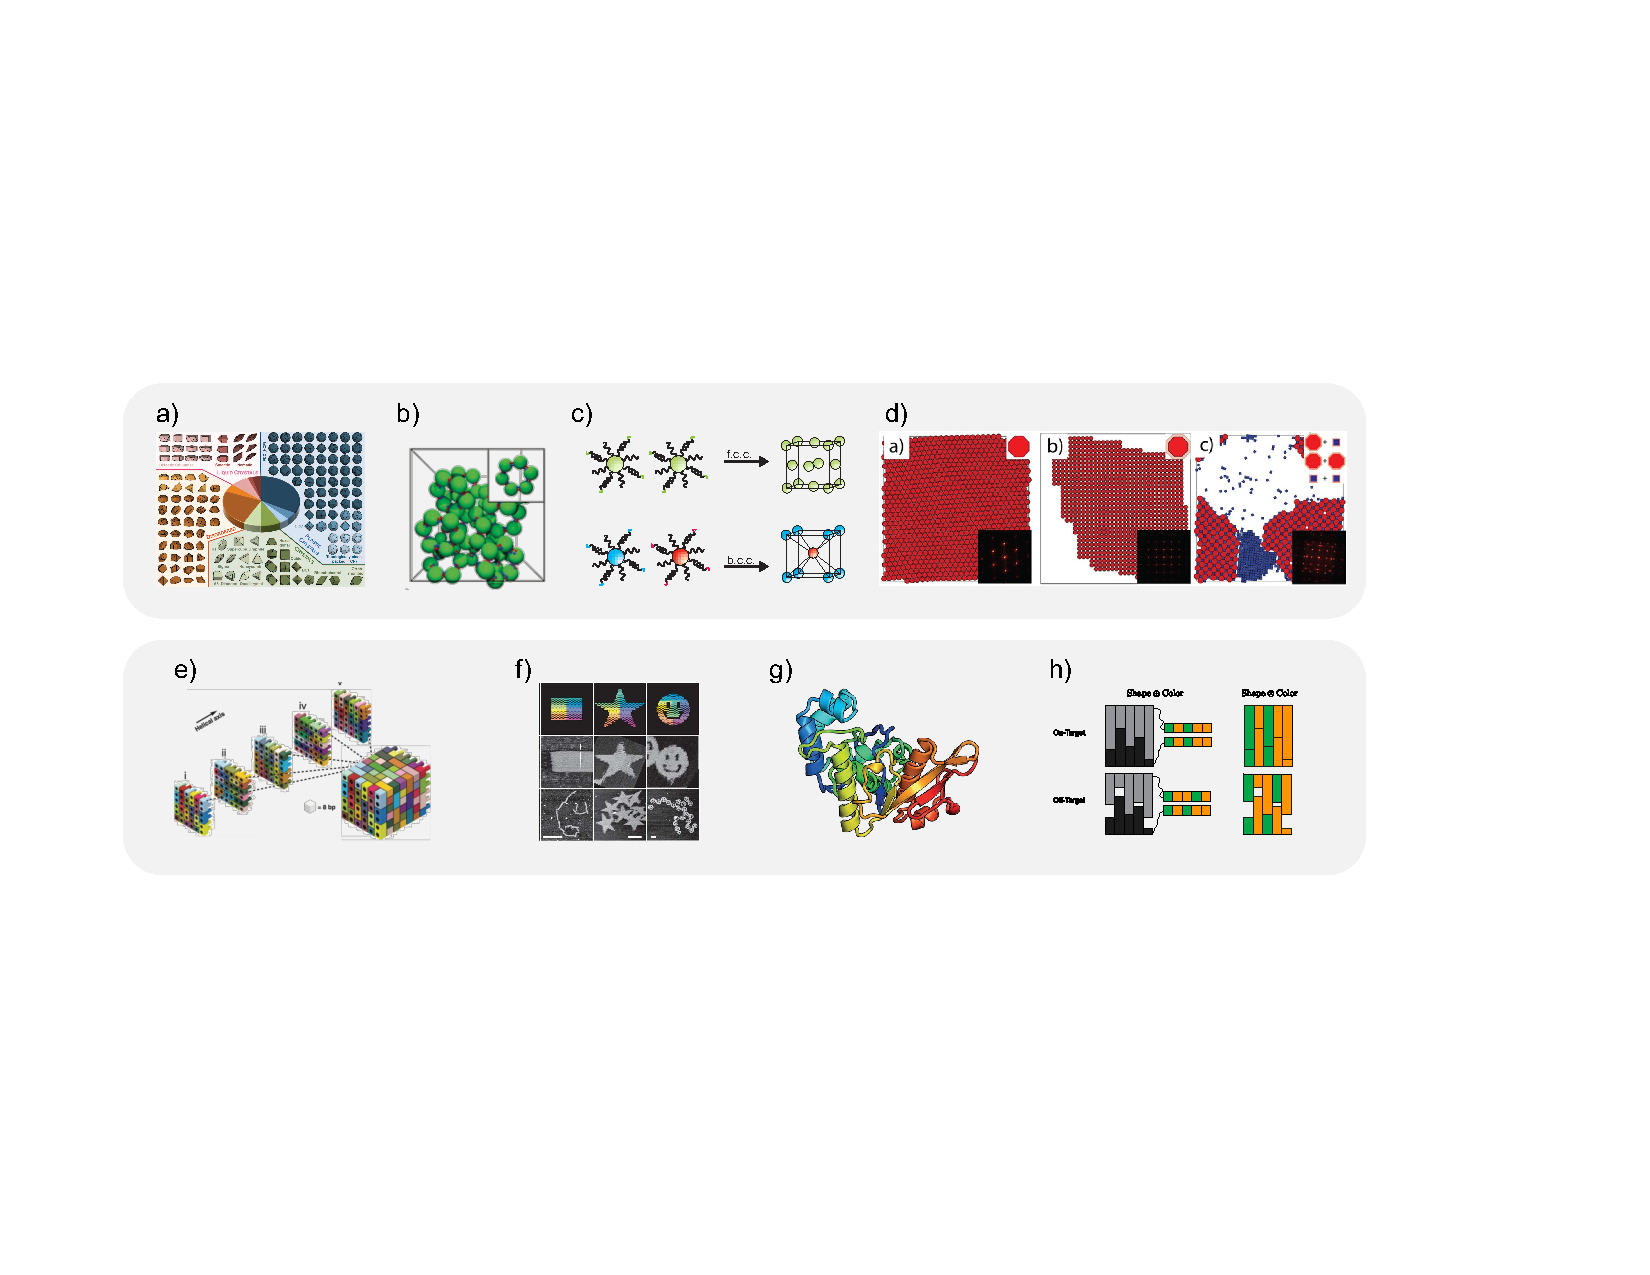
\includegraphics[width=6.5in]{../figures/1-LiteratureReview.pdf}
\caption{
\textbf{Self-assembly in the literature}:
Top: Simple interactions between particles can lead to a rich variety of assembled structures.
Systems shown: 
(a) ordered structures from hard polyhedra \cite{Damasceno_2012_Science};
(b) isotropic particles with attractive patches \cite{Zhang_2004_NanoLetters};
(c) crystal structure tailored with DNA-mediated assembly \cite{Park_2008_Nature};
(d) Archimedean tilings assembled from polygons with increasing bond specificity \cite{Millan_2014_ACSNano}.
Bottom: Programmable interactions can enable addressable complexity.
(e) DNA bricks assembled in a one-pot system with single-stranded DNA \cite{Ke_2012_Science};
(f) DNA origami \cite{Rothemund_2006_Nature};
(g) de novo protein design \cite{Huang_2016_Nature};
(h) theoretical calculation of chemical and shape bond instruction capacity \cite{Huntley_2016_PNAS}.
}
\label{fig:litreview}
\end{center}
\end{figure}

However, recent advances in synthesis of programmable DNA building blocks have now enabled significantly more complex interactions, resulting in self-assembly processes of addressable complexity.
In addressable systems, each particle has a specific location (address) that it is ``programmed'' to assemble into.
%Such assembly is as much a function of the kinetics of the process (e.g. annealing) as it is the thermodynamics of the interparticle interactions.

Biologically, we are familiar with specifically-programmed assembly in DNA replication or protein folding \cite{Dill_1993_CurrOpinStructBiol}.
Synthetically, though, the most well-known examples of addressable complexity are DNA-based.
``One-pot'' addressable self-assembly of DNA bricks uses the hybridization of complementary DNA sequences to construct addressable structures from a single pool of monomers \cite{Ke_2012_Science}.
Simulation results have shown that such one-pot self-assembly can succeed with highly simplified model subunits that lack the molecular details of DNA tiles, suggesting that similar design strategies should be possible in non-DNA-based synthetic systems \cite{Reinhardt_2014_PRL}.

In addition to using programmed DNA interactions between particles, programmed self-assembly can also refer to design of DNA strands or protein primary structures themselves.
DNA origami is perhaps the most well-known example of this \cite{Rothemund_2006_Nature,Winfree_1998_Nature}.
Given a target structure (such as the much-cited example of a smily-face), a DNA strand can be programmed that will fold precisely into the designed target \cite{Rothemund_2006_Nature}.
While some examples of protein design exist (e.g. \cite{Huang_2016_Nature}), it is possible that the additional challenge of designing structure from a set of 22 amino acid residues versus 4 nucleotide bases in DNA has limited its appeal as a designer system.

While much work has focused on designing interactions to tailor self-assembly, we must also note that simply having sufficiently-specific interactions does not guarantee a system will reach a target state.
If assembly temperature is too high, bonds may be unable to stably form; if the assembly temperature is too low, the system may be unable to sufficiently sample configuration space to reach the target structure.
Though the target maybe be the global free energy minimum, that does not mean that it can be reached kinetically.  
Temperatures and binding energies must be carefully tuned to enable systems to sufficiently sample possible configurations and escape kinetic traps while still enabling stability in the ground state (i.e. bonds do not spontaneously break).
In a noteworthy example, the yield of the one-pot DNA self-assembly system studied in \cite{Ke_2012_Science} was found via simulation to be highly sensitive to both temperature \cite{Reinhardt_2014_PRL} and the annealing protocol used \cite{Jacobs_2015_PNAS}. 

A collection of the self-assembly results discussed here and in the remainder of this proposal is shown in Figure \ref{fig:litreview}.


%\subsubsection*{Background}

Active matter has been a field of rapidly expanding interest and research activity over the last decade \cite{Ramaswamy_2010_AnnRevConMatPhys,MarchettiEA_2013_RevModPhys,BechingerEA_2016_RevModPhys,MarchettiEA_2016_CurrentOpinionColloidInterfaceScience}.
Vicsek's pioneering work showed that collections of point particles with alignment rules displayed rich collective behavior, including phase separation \cite{VicsekEA_1995_PRL}.
However, theoretical work seeking to describe the collective behavior of bacteria demonstrated that phase separation was not reliant upon explicit alignment rules \cite{Cates_2010_PNAS}.
Giant number fluctuations characteristic of phase separation in these systems of isotropic particles were found to lead to phase separation based on density-dependent slowing in a phenomena now known as ``motility-induced phase separation'' (MIPS) \cite{CatesTailleur_2013_EPL}. 
This phase separation in isotropic systems has been described as athermal phase separation \cite{FilyMarchetti_2012_PRL}, kinetic steady-state balancing of particle fluxes \cite{RednerEA_2013_PRE, RednerEA_2013_PRL}, classical nucleation \cite{Richard_2016_SoftMatter,Redner_2016_PRL}, and balancing of collision theory timescales \cite{Bruss_2017_arxiv}.
Importantly, this same phase separation predicted by theory has been observed in experiments, which confirm the activity-dependent formation of ``active crystals'' at low system densities \cite{PalacciEA_2013_Science,PetroffEA_2015_PRL}.

However, in real-world systems (e.g. bacteria) particles are rarely isotropic.
Simulations of rods with varying aspect ratios have been shown to display a rich variety of collective motion dependent on shape and system density \cite{WensinkLoewen_2012_JPhysConMat,YangEA_2010_PRE}.
Drawing from the example of anisotropic swimmers such as bull sperm and \textit{Chlamydomonas}, Wensink \textit{et al} observed that shape and direction of the translational driving force relative to the shape (referred to as ``force offset'' in this paper) allowed for differing modes of collective motion and onset of critical behavior \cite{Wensink_2014}.
Similarly, gear shaped ``spinners'' with differing directions of a rotational driving force were shown to phase separate through competing steric interactions (repulsive for opposite spinners, and attractive for like spinners) \cite{NguyenEA_2014_PRL, SabrinaEA_2015_SoftMatter, SpellingsEA_2015_PNAS}.
In a study of active dumbbells, Suma \textit{et al} noted that particle anisotropy allowed for stabilization of cluster rotation, a phenomenon not seen in clusters of isotropic particles \cite{SumaEA_2014_EPL}.
Finally, a study of active squares uncovered an ``oscillatory'' activity/density regime in which large clusters would break up and re-form at steady state \cite{PrymidisEA_2016_SoftMatter}. 

Why is a description of the role of active particle anisotropy needed?
We can view this spontaneous ``phase separation'' and organization as a type of non-equilibrium self-assembly \cite{Mann_2009_NatureMaterials}.
It is well established that in the absence of attractive forces in equilibrium self-assembly, shape alone is sufficient to determine the minimum free-energy structure \cite{Onsager_1949_ANYAS,Damasceno_2012_Science,Manoharan_2015_Science,vanAndersEA_2014_PNAS}. 
While self-assembling, fluctuations allow a system to randomly sample system configurations until it finds the one with the minimum free energy.
However, sometimes the global free energy minimum is kinetically difficult to reach, and the system can become kinetically trapped in a metastable state.
Activity provides a driving force which can help anneal a system out of these kinetic traps \cite{VanDerMeerDijkstraFilion_2016_SoftMatter,Mallory_2016_PRE} or stabilize system configurations that would be unstable without the additional driving force \cite{ZhangYanEA_2016_AngewandteChemie}. 
Understanding how particle anisotropy combined with an active force director will impact the collective motion, even in the form of a general heuristic, would open the doors to studying non-equilibrium self-assembly tailored through particle anisotropy. 

\begin{figure}[t]
\begin{center}
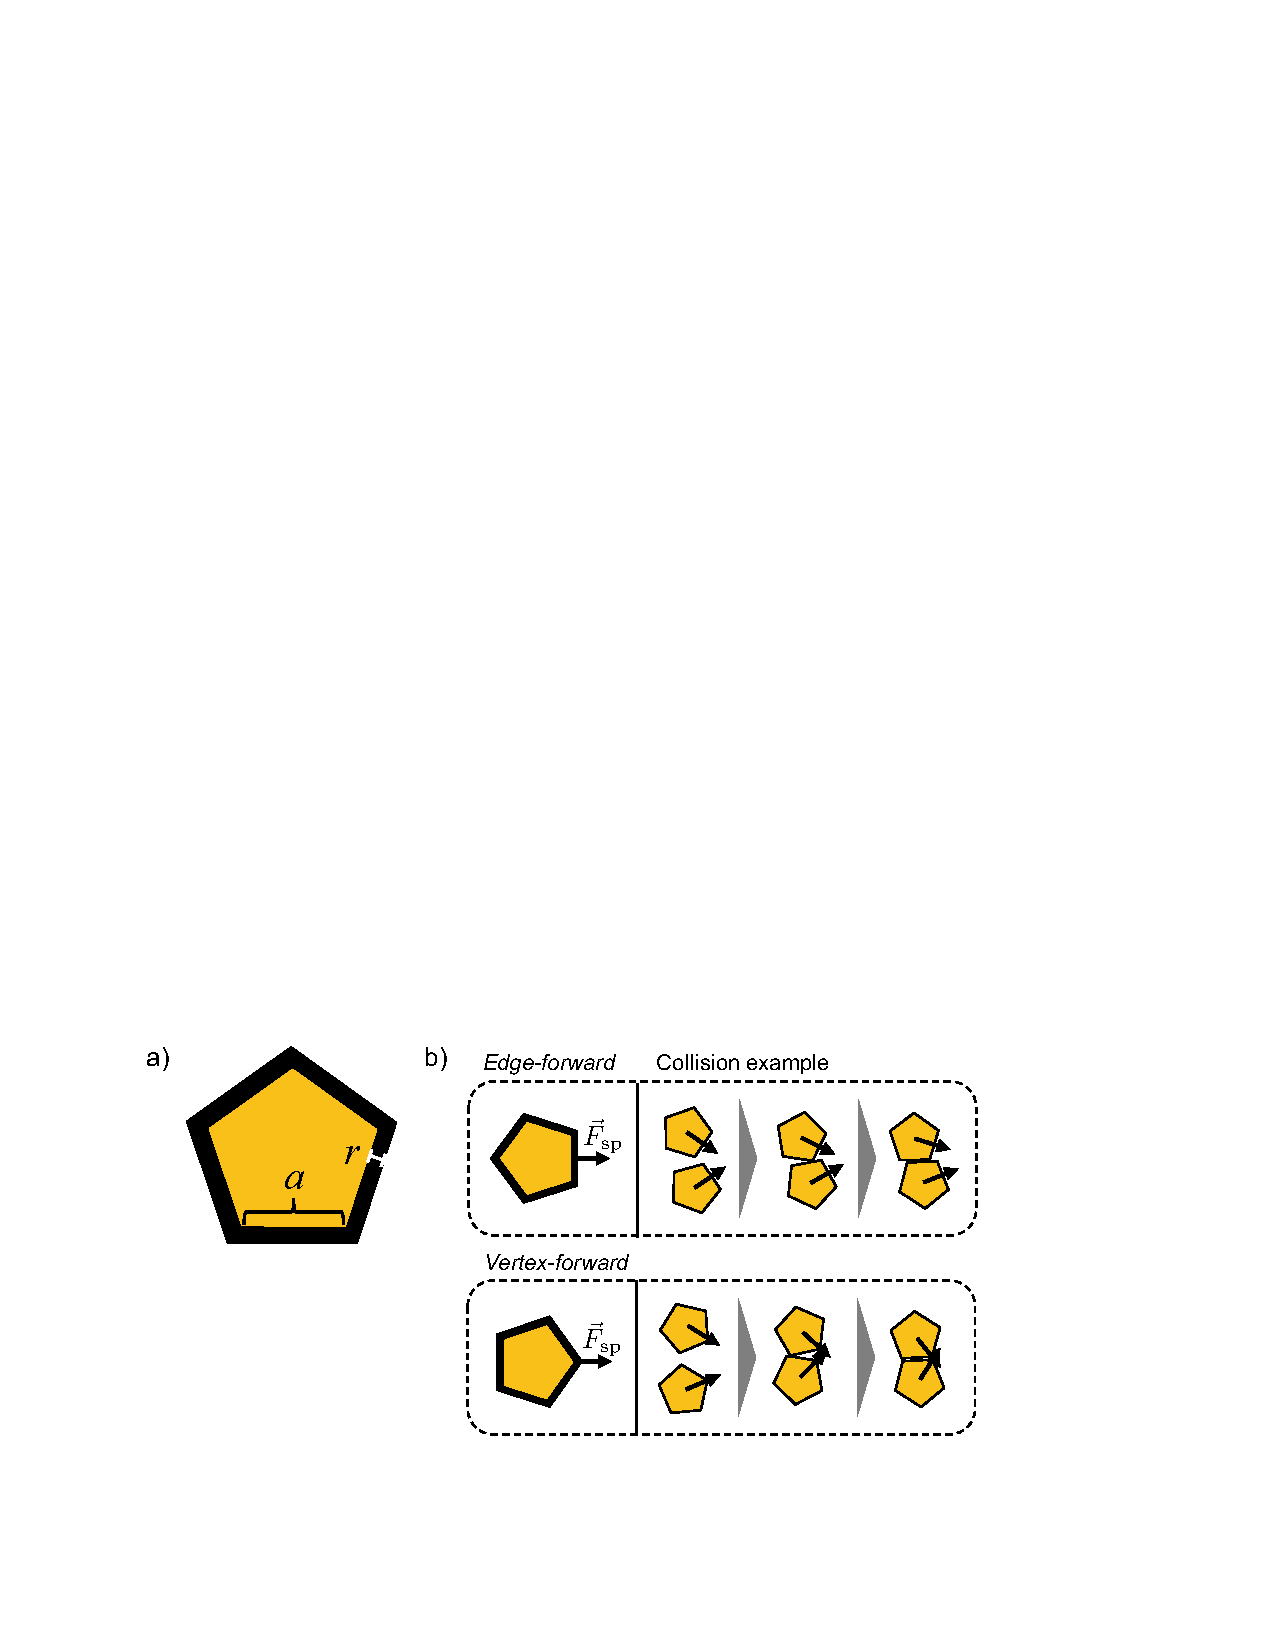
\includegraphics[width=4in]{../Figures/Fig1.pdf}
\label{fig:model}
\end{center}
\caption{
\textbf{Model system}:
(a) Shape anisotropy is studied with a family of regular polygons of side number $n=3-8$, characterized by side length $a$.
Particles interact through a purely repulsive WCA potential of radius $r=1$.
The dimensions of all shapes are set such that $\frac{n{\cdot}a}{2{\pi}r}=0.9$.
(b) Force anisotropy is implemented through the direction of the self-propelling force, which propels the shape either edge- or vertex-forward.
A key feature of this system is that collisions of anisotropic particles can sustain dimer (and larger n-mer) translational and/or rotational motion.
Illustrative collisions are provided for each force director.
}
\end{figure}

%In all studies of active shapes, some degree of particle ordering has been found in the clusters. 
To date, the differing behavior between active disks and active shapes has been explained in system-specific terms. 
Here, we study a system of active shapes to systematically understand and describe the role both shape and force anisotropy play in the collective behavior of translationally-driven active systems using the model shown in Fig. \ref{fig:model}.
Shapes are implemented using the discrete element method \cite{DEM_2017} implemented in HOOMD-blue \cite{HOOMD_2008, HOOMD_2015}.
We use Langevin dynamics to model the movement of the particles studied here, and take care to select a sufficiently small mass that the system is effectively Brownian, in line with the expected dynamics of bacteria.
Full simulation parameters can be found in the Methods section of the in-preparation paper.
% 1 page statement of the problem, purpose and significance of the research
%\section{Background}

\begin{figure}[t]
\begin{center}
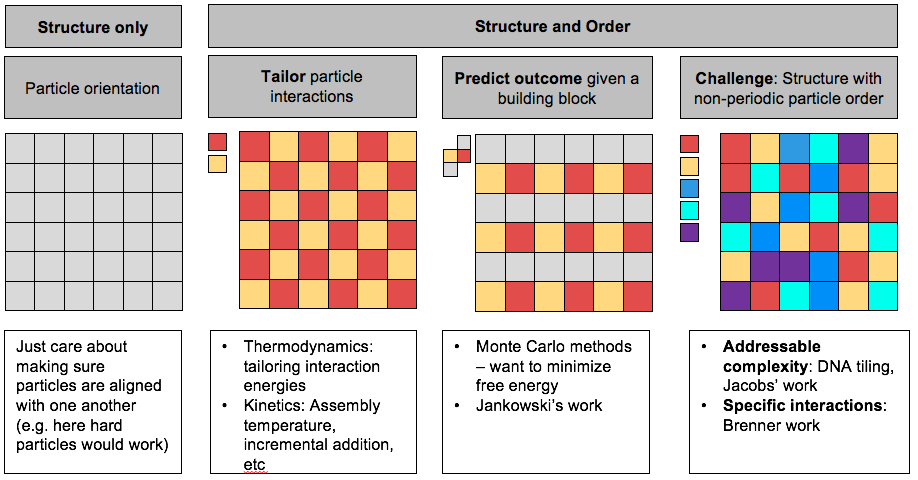
\includegraphics[width=6.5in]{../figures/litreview.png}
\caption{Demonstration of the state of the art in the literature}
\label{fig:litreview}
\end{center}
\end{figure}

Let's take a simple system and use it to illustrate the state of the art in the theory for engineering self-assembly behavior.

Let us say that we have the simple target 2D array shown in Figure \ref{fig:litreview}.

% =====
% STRUCTURE ONLY
% ====
\subsection{Directing structure}
If we assume all the particles in our system are uniform, we simply care about making sure particles assemble into the target structure.
As in any type of assembly, this implies a minimization of free energy.
In the example of hard squares above, minimization of free energy corresponds to a maximization of entropy.

\begin{itemize}
\item Archimedean tilings
\item Glotzer work on assembling target structures
\end{itemize}


\cite{vanAnders_2014_ACSNano}: Can treat shape as giving particles an effective entropic patchiness

\cite{Millan_2014_ACSNano}:
Develop a metric of self-assembly complexity, flow chart in Figure 3.
Archimedean tilings (ATs)
Here, we report the minimal set of interactions needed to self-assemble experimentally accessible ATs from regular polygons, mimicking nanoplates assembled into crystalline monolayers (Figure 1). We show through Monte Carlo simulations the self-assem- bly of these tilings by exploiting entropic and enthalpic interactions encoded in the shape of the polygons. We arrive at a design strategy for patchy polygon particles that is accessible to current experimental techniques and present the minimal set of design rules for each AT. We report that four ATs, namely, the (63), (36), (44), and (3.122) tilings, can be assembled solely with hard interactions, highlighting the role of directional entro- pic forces39,40 that arise from the particle shape.

After selecting the building blocks, the design pro- cess examined the constituent polygonal building blocks and alters the interaction complexity by chan- ging the specificity of interactions. The four models ranked in terms of specificity are hard, symmetric patches, shape-specific patches, and edge-specific patches

Manually adds complexity in the amount of specificity:
Initially, we test if entropic interactions are sufficient to self-assemble each crystalline structure. If the infinite pressure ground state (hard particle) won't assemble the target structure, add attractive interactions. If the crystalline structure for a mixture of building blocks does not contain the alternating building block property, it is necessary to use edge-specific interactions.


% =====
% STRUCTURE AND ORDER: TAILORING PARTICLE INTERACTIONS
% ====
\subsection{Directing structure and particle order}
As we look to make more complex materials, though, we also want to specifically order the particles within a structure.
We can approach this through tailoring the thermodynamics and/or the kinetics.

\begin{enumerate}
\item BUBBA work
\item DNA tilings / DNA origami
\item Protein origami
\item DNA-tailored assembly
\item need to find some other citations here?
\end{enumerate}

\begin{enumerate}
\item \cite{Jankowski_2009_JChemPhys,Jankowski_2011_JPhysChemB,Jankowski_2012_SoftMatter}
\item Design and self-assembly of two-dimensional DNA crystals \cite{Winfree_1998_Nature}, primer to DNA origami \cite{Castro_2011_Nature}, Programming Self-Assembly of DNA Origami Honeycomb Two-Dimensional Lattices and Plasmonic Metamaterials \cite{Wang_2016_JACS}, Designer nanoscale DNA assemblies programmed from the top down \cite{Veneziano_2016_Science}
\item Proteins can now also be designed, ala DNA origami: \cite{Huang_2016_Nature}
\item \cite{Mirkin_1996_Nature,Park_2008_Nature,OBrien_2016_JACS,Liu_2016_Nature}, DNA-guided crystallization of colloidal nanoparticles \cite{Nykypanchuk_2008_Nature}
\end{enumerate}


\cite{Park_2008_Nature}: can create crystals using DNA functionalization
\cite{OBrien_2016_JACS}: Colloidal crystallization can be pro- grammed using building blocks consisting of a nano- particle core and DNA bonds to form materials with controlled crystal symmetry, lattice parameters, stoichiometry, and dimensionality. Can tailor DNA length and shape to get different crystal structures

DNA programmable assembly. The sequence-specific binding property of DNA can be applied to direct the assembly behavior of colloidal particles at the nanoscale. This is a powerful strategy to control nanomaterial assembly because it allows tuning of the interparticle interaction in highly specific ways. For example, attaching DNA linkers with self-complementary sequences to particles directs them to maximize the number of nearest neighbors, resulting in fcc arrangement. On the other hand, particles with non-self-complementary linkers, which only allow A-B contacts, assemble into bcc or CsCl-type arrangement by maximizing the number of A-B contacts around the first coordination shell \cite{Park_2008_Nature}.This technique has recently been applied to anisotropic particles and opened possibilities to access diverse crystal structures in nanoscale by employing the DNA programmability as well as geometrical properties of the anisotropic shapes (25, 26).Despite its powerful potential, studies regarding the assemblies of DNA-coated anisotropic colloids have until recently (Sangmin's paper) been limited to simple crystal structures with small unit cells (27, 28). 

% =====
% STRUCTURE AND ORDER: PREDICTING ASSEMBLY
% ====
\subsection{Predicting assembly of complex building blocks}

Easy enough for hard particles, such as looked at in \cite{Damasceno_2012_Science}.
To test the interactions we've tailored above, we also need to be able to test the assembly properties of these building blocks.
We want to see what structure they will assemble into to minimize their free energy.
Our initial instinct would be to run these simulations to steady state or equilibrium.
However, systems with complex interactions such as these can get themselves caught in metastable free energy local minima that MC methods may not have large enough energy fluctuations to escape from.
This is where thermodynamics and kinetics really come to play together

\begin{itemize}
\item BUBBA work
\item Wales work (disconnectivity graphs) - more of the thermo
\item Kinetic pathway design - Frenkel, Jacobs
\item Connectivity graphs to show the order of assembly
\item Pathway assembly sampling
\item swear I read something earlier today about metastable/kinetic traps
\end{itemize}



% =====
% STRUCTURE AND ORDER: THE BIG CHALLENGE
% ====
\subsection{Challenge: Self-assembly of complex structures}

Real-world:
\begin{itemize}
\item Protein assembly
\item Complex DNA tiling, assembly - Mirken, Winfree, Rutherford, check semisynbio sources
\end{itemize}

\textbf{Motivation 1: DNA assembly, DNA tiles, DNA cubes}

Taken from intro of \cite{Reinhardt_2014_PRL}: \\
The observation by Ke et al. [Science 338, 1177 (2012)] that large numbers of short, predesigned DNA strands can assemble into three-dimensional target structures came as a great surprise, as no colloidal self-assembling system has ever achieved the same degree of complexity.
That failure seemed easy to rationalize: the larger the number of distinct building blocks, the higher the expected error rate for self-assembly.
The experiments of Ke et al. have disproved this argument.
Here, we report Monte Carlo simulations of the self-assembly of a DNA brick cube, comprising approximately 1000 types of DNA strand, using a simple model.
We model the DNA strands as lattice tetrahedra with attractive patches, the interaction strengths of which are computed using a standard thermodynamic model.
We find that, within a narrow temperature window, the target structure assembles with high probability.
Our simulations suggest that misassembly is disfavored because of a slow nucleation step.
As our model incorporates no aspect of DNA other than its binding properties, these simulations suggest that, with proper design of the building blocks, other systems, such as colloids, may also assemble into truly complex structures.


\textbf{Motivation 2: Protein folding}

\subsection{Theory perspective}:
\begin{itemize}
\item Addressable complexity
\item Efficiency of specific interactions
\end{itemize}

From \cite{Wales_2017_JChemPhys}:
To construct an operational machine, we generally need to assemble a variety of components into a well-defined spatial arrangement. The experimental realisation1 of programmed self-assembly for a structure composed of thousands of dis- tinct building blocks has therefore generated great interest. Here the building blocks are ?DNA bricks,? which can bind by hybridisation to four neighbours. The resulting assemblies are considered ?addressable,? in that the different components are located in specific local environments. Understanding and developing design principles for such structures could pro- vide a route to translation of information encoded in nanoscale building blocks into new materials with a specific structure and function. Developing models that reproduce the key exper- imental results using the simplest possible representations is therefore an important challenge, and initial efforts for DNA bricks have already reproduced addressable assembly for as many as 1000 distinct components.2 Recent insight into computer simulation indicates that robust self-assembly may require precise conditions for nucleation to occur. The yield for the target structure can be improved significantly using a specific annealing protocol.3

\textbf{Information as a measure of the likelihood of a particular configuration being preferred.}
In 2015, a review article in \textit{Nature Physics} (which has since been cited 255 times) reviewed the state of the art on applying information theoretic entropy-- i.e. Shannon entropy-- as a way of understanding non-equilibrium thermodynamics \cite{Parrondo_2015_NaturePhysics}.
In this work, they investigate information entropy as a placeholder for non-equilibrium entropy production.
This entropy production gives an overall likelihood of a configuration (one which minimizes the non-equilibrium free energy of a system while maximizing the non-equilibrium entropy).
However, this method applies to the overall structure, or the overall likelihood of a structure being the preferred structure.

Some authors have gone so far as to suggest replacing the thermodynamic concept of entorpy with information \cite{AFarewelltoEntropy}.

\textbf{``Addressable complexity'' seeks to engineer pathways for particular particles to reach their destination.}
Low free energies of a target structure, however, do not guarantee efficient assembly.
There are a number of ways addressing this problem in the literature.
One way of forcing systems into assembly is to design a free energy landscape that minimizes such meta-stable traps \cite{Wales_2017_JChemPhys}.
Competition between degenerate structures of equivalent potential energy was reported for clusters of six attractive spherical colloids, where symmetry breaking leads to higher rotational entropy of the less symmetric conformation, resulting in lower free energy \cite{Meng_2010_Science}.

Taken from \cite{Jacobs_2015_JChemPhys}: 
A well-known example of addressable complexity-- that is, specific binding-- can be found in ``one-pot'' DNA self-assembly of DNA tiles, which use the hybridization of complementary DNA sequences to construct complex structures consisting of hundreds of subunits from a single soup of monomers \cite{Ke_2012_Science}.
Simulation results have shown that such one-pot self-assembly can succeed with highly simplified model subunits that lack the molecular details of DNA tiles, suggesting that similar design strategies should be widely applicable \cite{Reinhardt_2014_PRL}.
In the work by Jacobs \textit{et al}, they had particles with designed interactions between one another.
They represented the target bonds by a graph, $G$.
However, this model is based on the assumption that ``designed interactions in the target structure are typically much stronger than any incidental associations between sub-units that should not be connected in the final assembly''.
This is a fine assumption for their proof of concept, but is not valid in real-world system.
As a concrete example, protein-folding is perhaps the most well-explored biological system that assembles due to specific interactions \cite{Dill_1993_CurrOpinStructBiol}.
However, one of the major challenges to solving the protein-folding problem are competing ``cross-talk'' interactions [CITATIONS NEEDED; chaperoned folding and assembly Chakrabarty 2017].

In later work, Jacobs et al addressed this oversight and accounted for incidental interactions in addition to designed interactions \cite{Jacobs_2015_PNAS}.


Low energies may not guarantee efficient assembly
compartmentalized, multi-stage assembly
grannemana and baserga 2004

Talk outline:
1. self-assembly kinetics can be rationally designed-- leverage thermodynamics
2. evolution has already selected for optimal assembly pathways in complex biomolecules


\textbf{Specific binding interactions can be tailored to lead to target structures}.
However, there is a delicate balance of specificity required.
On the over-specified side, we have bonds that are specific to their intended neighbor with probability 1.0.
On the under-specified side, we have non-specific interaction patches that will bond to any other patch with probability $1/n$, where $n$ is the total number of patches in the system.

In work from our group, Eric Jankowski sought to generate energy-minimizing configurations for such patchy particles \cite{Jankowski_2009_JChemPhys} in a process he called ``bottom-up building block analysis'', or BUBBA.
Cluster Monto Carlo (cMC) and LAcMC methods are relatively poor methods for finding potential energy minima formed from patchy particles with disparate interaction energies due to their tendency to become trapped in metastable configurations as well as the low degeneracy of potential energy-minimizing configurations (Q).
BUBBA effectively searches a subset of the configuration space for energy-minimizing configurations.
Jankowski predicted that that BUBBA would be useful for evaluating many different particles for self-assembly ``propensity''.

Partition functions encode all the thermodynamics of a system, but for most systems of practical importance they cannot cannot be calculated exactly.
This is due to many indistinguishable degenerate states. 
In the cases where small numbers of distinguishable configurations comprise a majority of a partition functions' weight, as is the case for systems at low temperatures and for many anisotropic building blocks with disparate interactions, BUBBA is a particulalry effective method for generating partition functions that have been heretofore inaccessible. 
This allows us to ask ``What structures are thermodynamically favored for this building block at any temperature?'' to be answered independently of assembly kinetics. \cite{Jankowski_2011_JPhysChemB}

% Note: Jankowski_2011_JPhysChem has a really good introduction

Both thermodynamic and kinetic barriers to assembling target structures.

Let's first look at a paper from the Brenner group, the ``Information capacity of specific interactions' \cite{Huntley_2016_PNAS}.
Their main thesis is that specific binding interactions have energetics that allow binding to occur with measurable probability.
Thus, we can measure the relative information in different types of binding.
This is more in line with the communication theory view of information (rare events giving more information) than it is with the materials view of information, in which high information events imply high probability of a desired event happening.

Our group, and many others in the materials community, are looking to engineering materials to control their structures, behaviors, etc.
A common method of engineering these materials is by tailoring the interactions between their components through chemistry, shape, etc.
By understanding how much \textit{assembly information} can be contained in these interactions, we can:
\begin{enumerate}
\item Compare the efficacy of different types of interactions in delivering desired behavior(s)
\item Theoretically predict the efficacy of new types of interactions
\end{enumerate}

Let's take the example of a lock and key system.
\textcolor{red}{ADD SECTION ON BRENNER PAPER FROM LIT REVIEW LAST YEAR}

However, we can use the concept of \textit{mutual information} in defining how much information is stored in an interaction in an intuitive manner.
(See notes on the Brenner paper below.)
Mutual information $I(X;Y)$ is a global measure of interaction specificity in systems with many distinct species.
It quantifies how predictive the identity of a lock $x_i$ is to the identity of key $y_i$ found bound to it.


% Literature survey and description of research already performed by the applicant

% =====
% RESEARCH PROPOSAL
% =====
% section, each project is a subsection
\section{Description of proposed research (7-8 pg, 2-3 pg per aim)}
% Including method or approach and expected difficulties
% This must constitute about 50\% of the text of the written proposal: 7-8 pages
% Clear statement of the work to be undertaken and must include:
% Objectives for the period of the proposed work and expected significance
% Relation to the present state of knowledge in the field and to work in progress at Michigan/elsewhere
% Expected research program sequence
% Decision points expected during the course of the research
% Methods of data reduction, evaluation, interpretation and presentation

``Information'' are those factors that impact the yield and kinetics of self-assembly (thermodynamics of the free energy landscape and the kinetics of the path to get to a target structure from a given starting point).

Specifically, as we look to both understand how nature governs self-assembly into target structures, we need a language to understand this.`
Nature is very good at already picking an optimized route through a free energy landscape \cite{Jacobs_2016_BiophysicalJournal}.

\subsection{What I want to accomplish in my thesis}

1) Can we figure out which bonds/interactions are the most critical in an assembly process or an assembly pathway?
We intuitively know that in 
Need transition state or pathway sampling methods (or might actually be able to get this just from Paul?s data? That would be sick)

2) With this metric, can we then define and minimize an information efficiency, e.g. the amount of bond specificity we need across the system to get a given success rate of assembly?
E.g. is it more efficient 
3) Given all this, can we then use machine learning to determine a priori the ?most efficient? level of specificity for self-assembling a target structure?
How to do pathway design is kind of an open question
We can find feature correlations, like Paul did
There?s also an approach called ?Computable Information Density? published by some colleagues (Chaikin) on the arxiv last August
Basic idea is that you can (1) somehow represent your system as an array of information which you can (2) run though a compression algorithm and (3) the ?information? is just the length of that compressed information
Would be really interesting to see if I could extend that idea to the features of an assembly system? in this case, nets? and 


1) Define a measure of pathway information. \\
\begin{itemize}
\item We already have ways of measuring how good a particular bond is
\item Are there particular bonds/connections that are the most important to get correct to enable forming the desired final structure?
\item  
\end{itemize}



2) Use that measure of pathway information to design ideal pre-cursors for target structures. \\



3) Attempt to use machine learning to predict ideal pre-cursors for given target structures. \\
\begin{itemize}
\item \cite{Long_2014_JPhysChemB}: Nonlinear Machine Learning of Patchy Colloid Self-Assembly Pathways and Mechanisms out of the Furguson group
\end{itemize}


4) Why is it important we find the ``most important'' pathway points? from \cite{Stern_2017_arxiv} \\
How then can self-folding origami be folded with a
minimal number of actuators? A lesson can be drawn
from similar glassy landscape search problems in models
of protein folding (e.g., Levinthal?s paradox [17, 19, 20,
41]) and related NP-hard satisfiability (SAT) problems
[21, 42] that vary from the Traveling Salesman Problem
to Sudoku [43]. A common element in these satisfiability
problems is that random seeding of the search for
the global minimum leads to repeated backtracking after
reaching local minima, both in the context of computer
algorithms (as the DPLL algorithm for k-SAT [21]) or for
physical dynamics (as in protein folding) [42]. However,
careful seeding of the search - e.g., if the right boxes are
filled in first in Sudoku [43] or if the right parts of the protein
are folded first - can greatly reduce or even eliminate
backtracking [21] before reaching the global minimum.
Correct seeding is even more critical for origami since
folding is assumed to happen at ?zero temperature? (e.g.,
without any noise or fluctuations). As a result, the structure
cannot backtrack out of a local minimum as in the
case of non-zero temperature SAT problems [42].

This reference also has a really good introduction section relating origami and self-assembly \cite{Stern_2017_arxiv}.


% =====
% PRIOR WORK: SEMISYNBIO PROPOSAL
% =====
% subsection
%\subsection{Collaboration: Synthetic biology memory}

The below was a response to an NSF call for proposals for a Semiconductor Synthetic Biology.

We proposed using DNA-mediated assembly to store information in nanoparticle arrays.

Specifically, this is an example of addressable complexity, then trying to engineer how to get the particles to where they should go in the most energetic and information/complexity-efficient manner possible.


\textit{From intro}:
In Aim 1, we will investigate monomeric block formation, exploring the self-assembly of arbitrary geometric DNA objects with incorporated optical elements that can be manufactured as information carriers, while allowing for superstructure formation through DNA-sequence barcoding. We will explore static assembly of 1D arrays of such DNA nanoparticles integrated with Memory Blocks (DNAMB) for encoding bitstream information that can be read out by fluorescence and electron microscopy. In Aim 2, we will explore 2D and 3D assembly, investigating techniques to algorithmically assemble and read out digital 2D and 3D information using optical and tomographic methods. In Aim 3, we will use molecular decision computing to assemble distinct, alternative lattices based on specific external signals. These results will offer the ability to encode and decode arbitrary datasets in ultra-dense molecular hard-drives, with environmental sensing and recording.

Aim 2. Dense, programmable molecular memory in 2D and 3D bit module lattice assemblies
Overview \& Rationale. Nanoparticle self-assembly depends on a balance of interaction forces, entropic effects, and system kinetics37,53,69-73. We can leverage these properties to direct self-assembly of shaped DNA nanoparticle into 2D and 3D arrays by controlling the position and valency overhangs that provide connectivity between DNA nanoparticles. Wireframe structure of DNA particle is highly suitable for encapsulation of memory blocks (e.g. Au NP, QDs, fluorescent dyes) and creation of DNAMB, a pixel in 2D or 3D arrays. To achieve information storage capabilities, it is required to investigate how the connectivity properties of DNAMB can be translated into their designed arrangement in the information- storing arrays. To self-assemble these systems into 2D and 3D ultra-dense data blocks, we will investigate the minimum interaction specificity needed to direct self-assembly into high fidelity ordered 2D and 3D arrays. We will also explore information retrieval from these arrays in 2D and 3D within pixels consisting of 1x1, 2x2, 4x4, etc., nanoparticle block arrays. In addition, we will establish methods for generating robust memory arrays that can preserve information under extreme conditions.

\textit{Proposed research, Aim 1}: Computationally, Glotzer and colleagues will develop a bit module interaction model to study the role of the DNA linkages on DNA cage self-assembly. Specifically, previous work on modeling solid particles with DNA-facilitated attraction37 will be extended to model the DNA cages that will be experimentally made by Gang, and it will consider realistic features of nanoparticle systems82,83. With this model in place, we can then extend the framework of digital alchemy, which treats particle properties as a thermodynamic variable, to particle interactions (here, DNA linkages)54. In this way, we can inversely design ideal DNA cages (e.g. shape, patchy interactions) that will robustly assemble a target structure. We will seek to balance site specificity without being overly unique?that is, design the highest information interactions that will allow for the minimum amount of linkage specificity for directing self-assembly84,85. This computational framework for the inverse design of bit packages that will assemble a given structure will enable high- throughput screening of particles of interest and serve as the basis for complex hierarchical structure and array assembly in the remainder of Aims 2 and 3.

Sub-Aim 2.2. Hierarchical assembly logic for higher-dimensional information storage
Overview. In Sub-aim 2.1, we explored approaches to assembling DNA frames into target 2D and 3D assemblies. Next, we precisely order ?bit modules??that is, DNA cages carrying functional particles? into arrays of discrete information. Toward this end, we design modules that carry the minimal information needed to reach target arrangements through a combination of particle anisotropy and DNA linkers. DNA
 computing groups have previously used DNA linkers to self-assemble complex 2D patterns6 and 3D shapes9. Here we extending these approaches to realize hierarchical 3D nanoparticle assembly design so that pixelated images act as dense data storage units. We will explore several complementary approaches to hierarchical assembly engineering, including sequential nanoparticle addition and ?one-pot assembly?, each of which will be explored together with inverse computational design of self-assembly pathways and particle geometries to achieve a robust assembly of designed arrays. Using the optical characterization strategies from Sub-aim 2.1, we will decode the information encoded in the structure, and probe sources of error and information loss in the self-assembly and read-out processes.

\textit{Proposed research}. Assembly of encoded 3D arrays can be approached in two strategies, or a combination thereof (Fig. \ref{fig:semisynbio}). In an entirely ?one-pot? assembly of a 3D array, all modules are linked with a large binding sequence set that has been fully computationally defined. Such an approach requires an enormous number of unique binding sequences, and even if fully defined, can run into high error rates when considering the assembly and packing of large (as compared with molecular assembly) and charged modules and/or materials. A second approach using sequential binding based on module groups of similar binding layouts requires less sequence diversity and can be automated using robotic liquid handling. However, this is vastly more process- and time-intensive than one-pot assembly. This approach represents hierarchical assembly, whereby 1D structures (?strings?) would be formed from the modules, 2D planes formed from the 1D libraries, and finally 3D encoded arrays from stacking of selected planes. An optimal assembly process that balances fully-encoded organization with direct addition of binding components would offer a hybrid approach of hierarchical assembly with sequential addition of groupings of computationally defined structures. Each of these strategies will be explored in this aim, using a combination of high-throughput, structure-based computational modeling and experiments.

The Glotzer group will extend their digital alchemy framework to probe diverse DNA linkage sequences and conjugation designs to realize specific, targeted inter-particle interactions. In addition, they will explore the roles of these interactions on the kinetics of array assembly to enable pathway design \cite{Jankowski_2012_SoftMatter} into desired arrays while avoiding undesirable ?side products?. In this way, we will explore computationally the interplay between the two extremes of one-pot and sequential assembly, and identify which combinations provide lowest assembly error while minimizing both assembly time and the number of required unique binding sequences. The Gang group will employ a home-built robotic system for automatic synthesis and assembly of DNAMB; that will allow establishing practical methods for creation of large number of diverse blocks required for the hierarchical assembly. While such approaches have been applied to molecular systems, they have not yet been realized for DNA frames integrating inorganic NP. To implement complementary pathway design strategies, Gang will fabricate DNA frames with thermally differentiated inter-vertex hybridizations to promote highly specific assembly path during thermally-driven self- assembly. For example, DNAMB strings will be assembled at higher temperatures, and planar and 3D arrays assembled at lower and lowest temperatures, respectively. We will use SAXS and tomography methods to reveal the pathway-controlled assembly process. The computational design of frames and pathways will be performed jointly between the Bathe, Glotzer, and Gang labs.

\begin{figure}[t]
\begin{center}
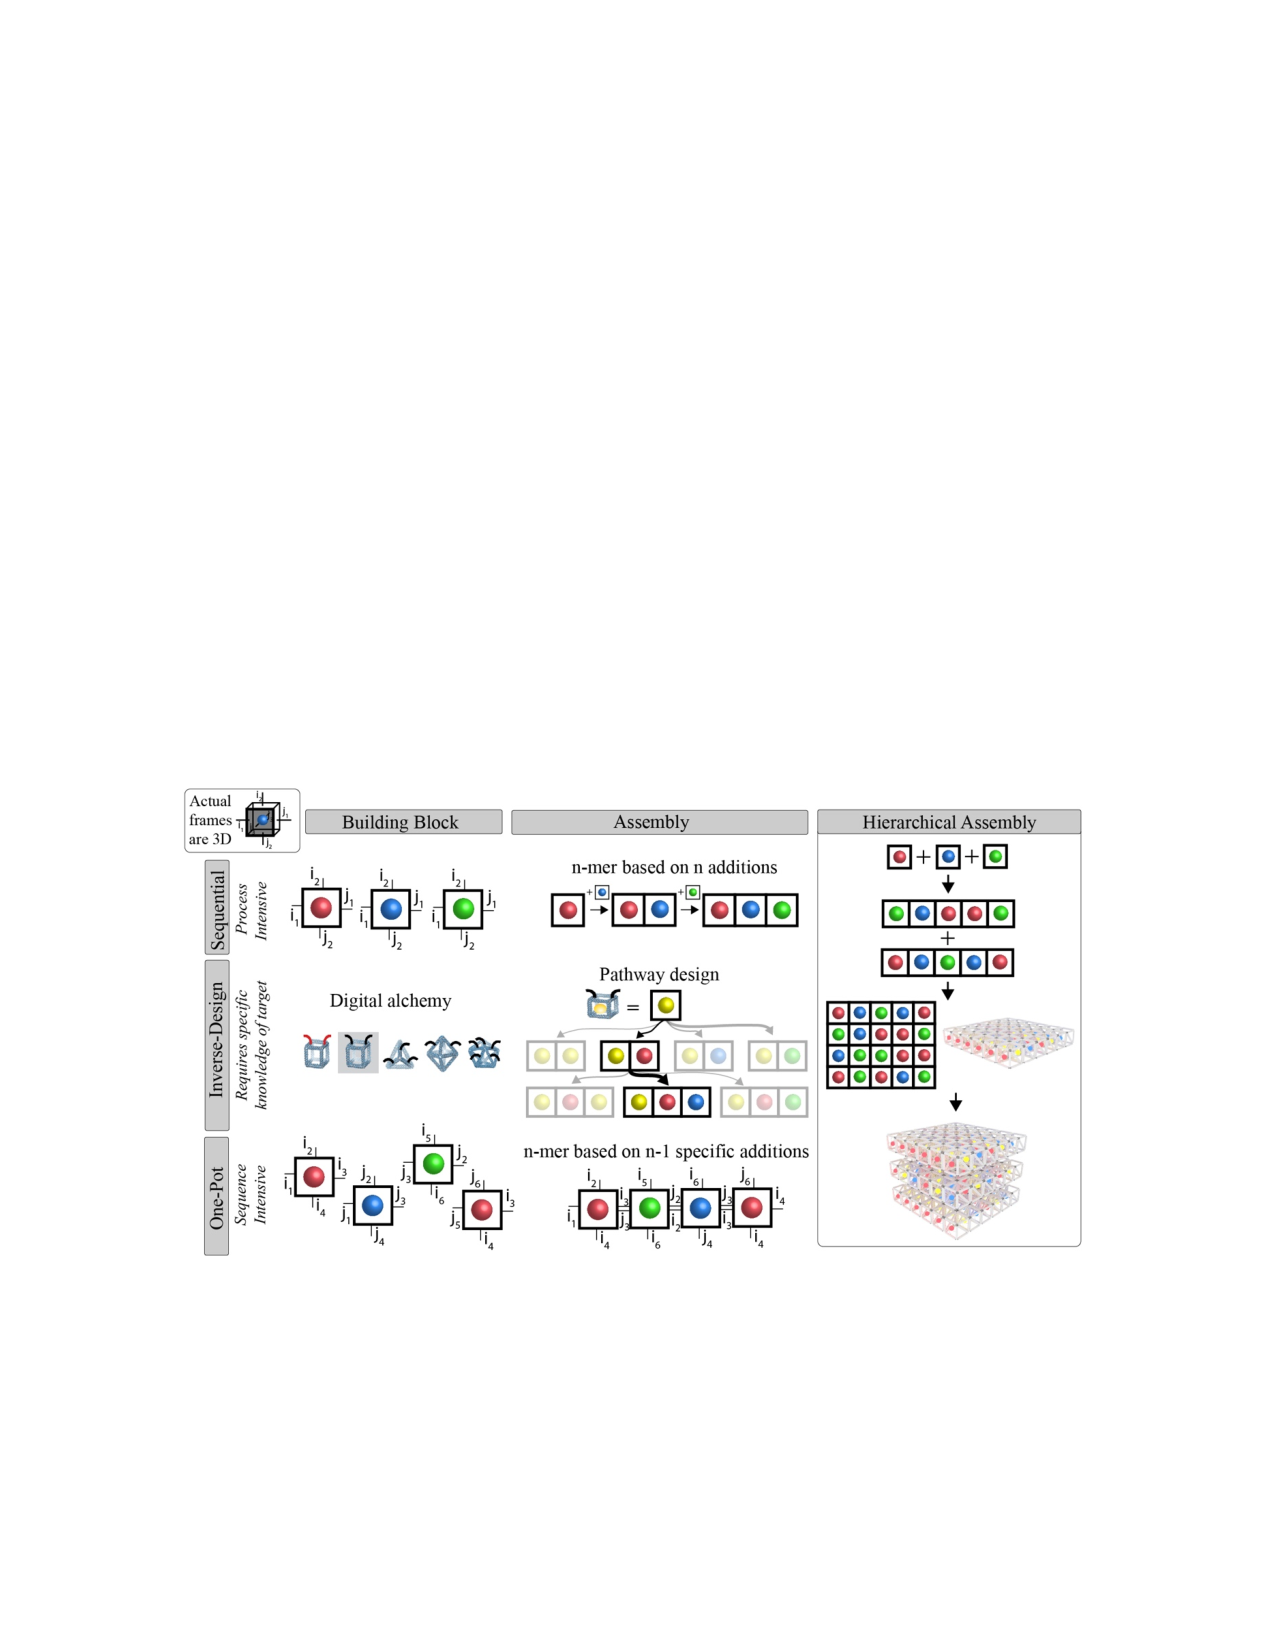
\includegraphics[width=6.5in]{../figures/SemiSynBio.pdf}
\caption{
(Lifted from SemiSynBio Proposal) Strategies for building information encoded 1D, 2D and 3D arrays. Sequential operations are very deterministic and can be carried out by automated robotic equipment, but even so are heavily process intensive and require many individual assembly steps. One-pot systems can be fully computationally defined, though in practice are heavily sequence intensive and be subjected to errors more readily than in molecular- scale systems when accounting for kinetic and thermodynamics of packing larger objects and materials. A hierarchical assembly methodology offers a hybrid approach of both strategies, where a sequential addition of structures preformed in a one-pot setup provide the desired 3D material organization.}
\label{fig:semisynbio}
\end{center}
\end{figure}

% =====
% PRIOR WORK: ACTIVE SHAPES
% =====
% section, previous work
%\section{Prior work: Leveraging anisotropy for tailoring self-assembly in active systems}

The following is taken from an in-preparation manuscript. \cite{Moran_2018_unpublished}

\textbf{Relation to proposed thesis topic}: If we define information broadly as any quality of a building block that impacts the emergent behavior of a system of those particles (in this case, force direction and shape), then we can argue this work is looking at a few aspects of information in active systems.


\subsection{Background}

\subsection{Methods}

\subsection{Results}

\subsection{Next steps}


\begin{figure}[t]
\begin{center}
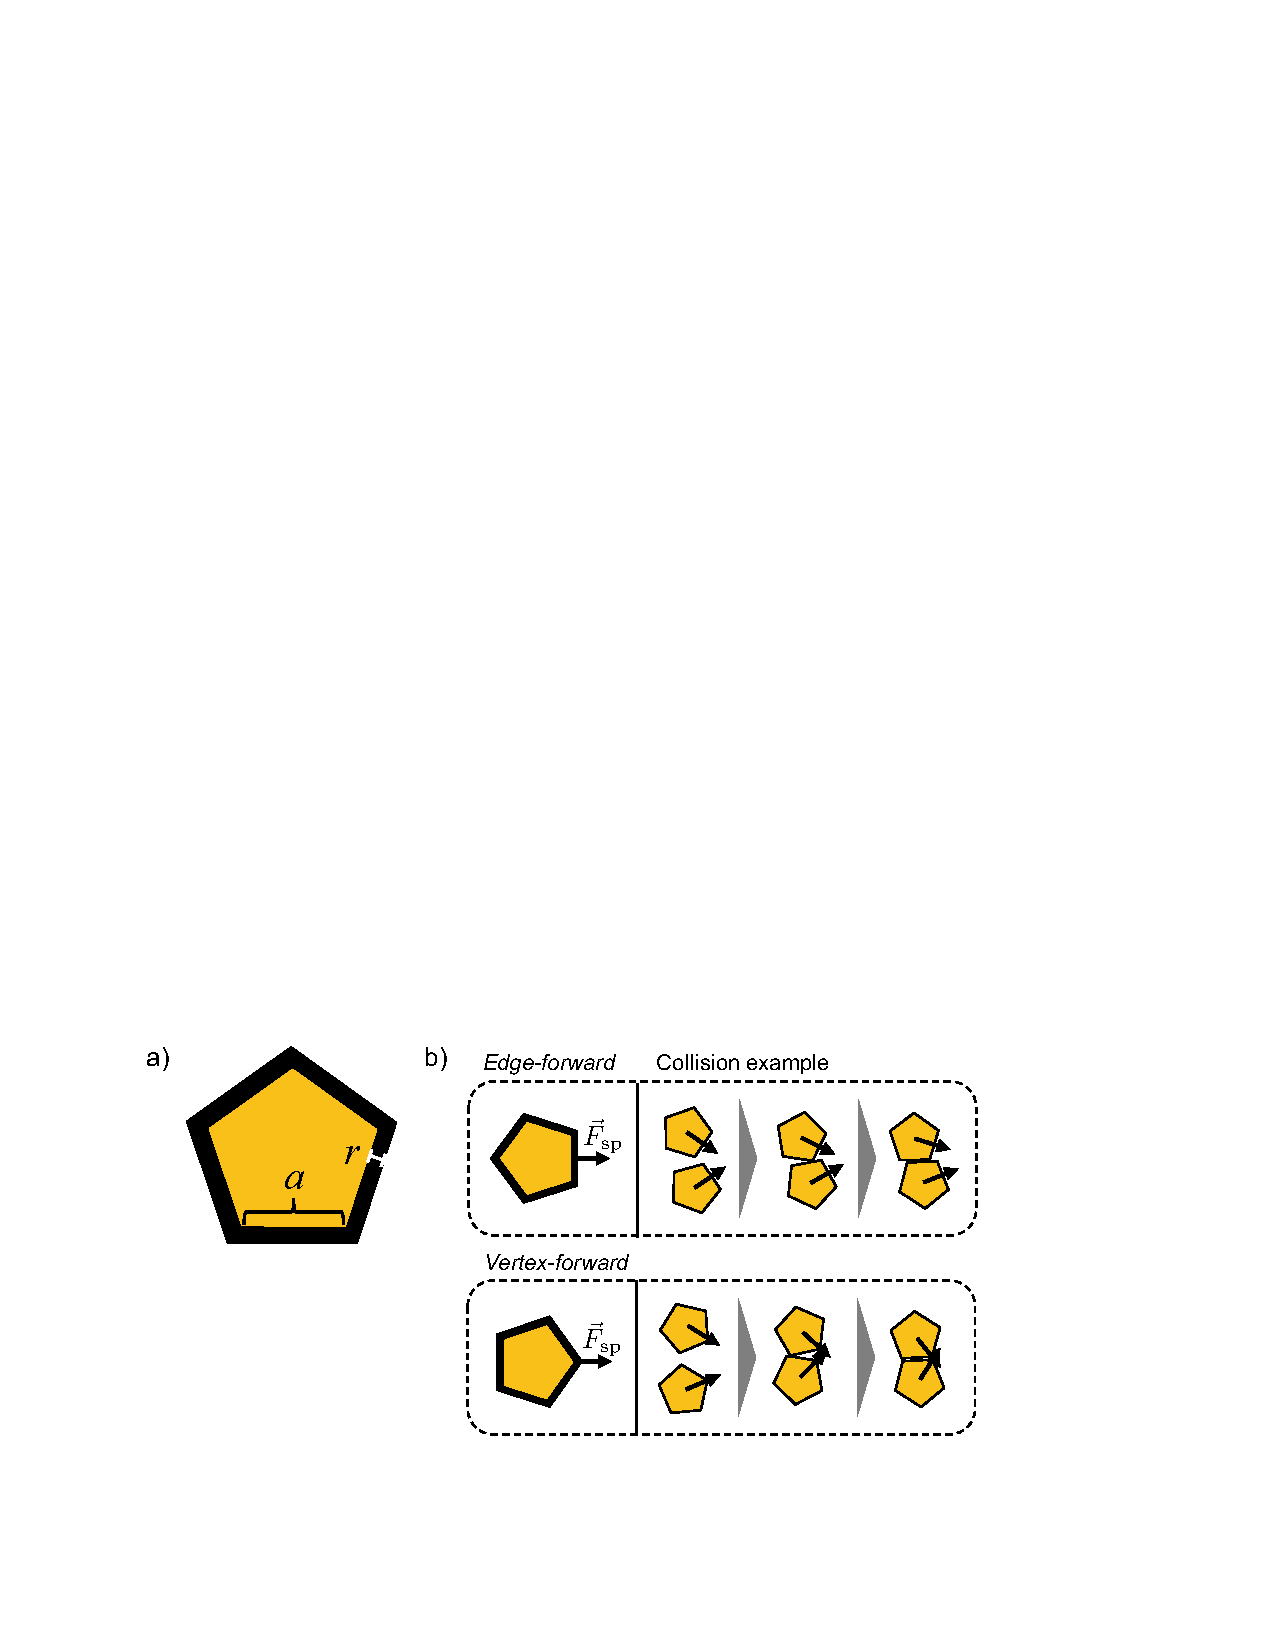
\includegraphics[width=5in]{../figures/Fig1.pdf}
\caption{\textbf{Model system}: (1) We use rounded shapes of constant S-C ratio, where the corners are rounded by a WCA potential, to ensure we can distinguish between shape steric (anisotropic) effects and isotropic behavior; (2) Force can be applied either perpendicular to the face or directed out a corner}
(Qs) should all particles be the same size?-- can't be, the way it's set up; all particles have drag of an equivalent disk; should we neglect noise? what does that mean for these simulations?
\label{fig:model}
\end{center}
\end{figure}

\begin{figure}[t]
\begin{center}
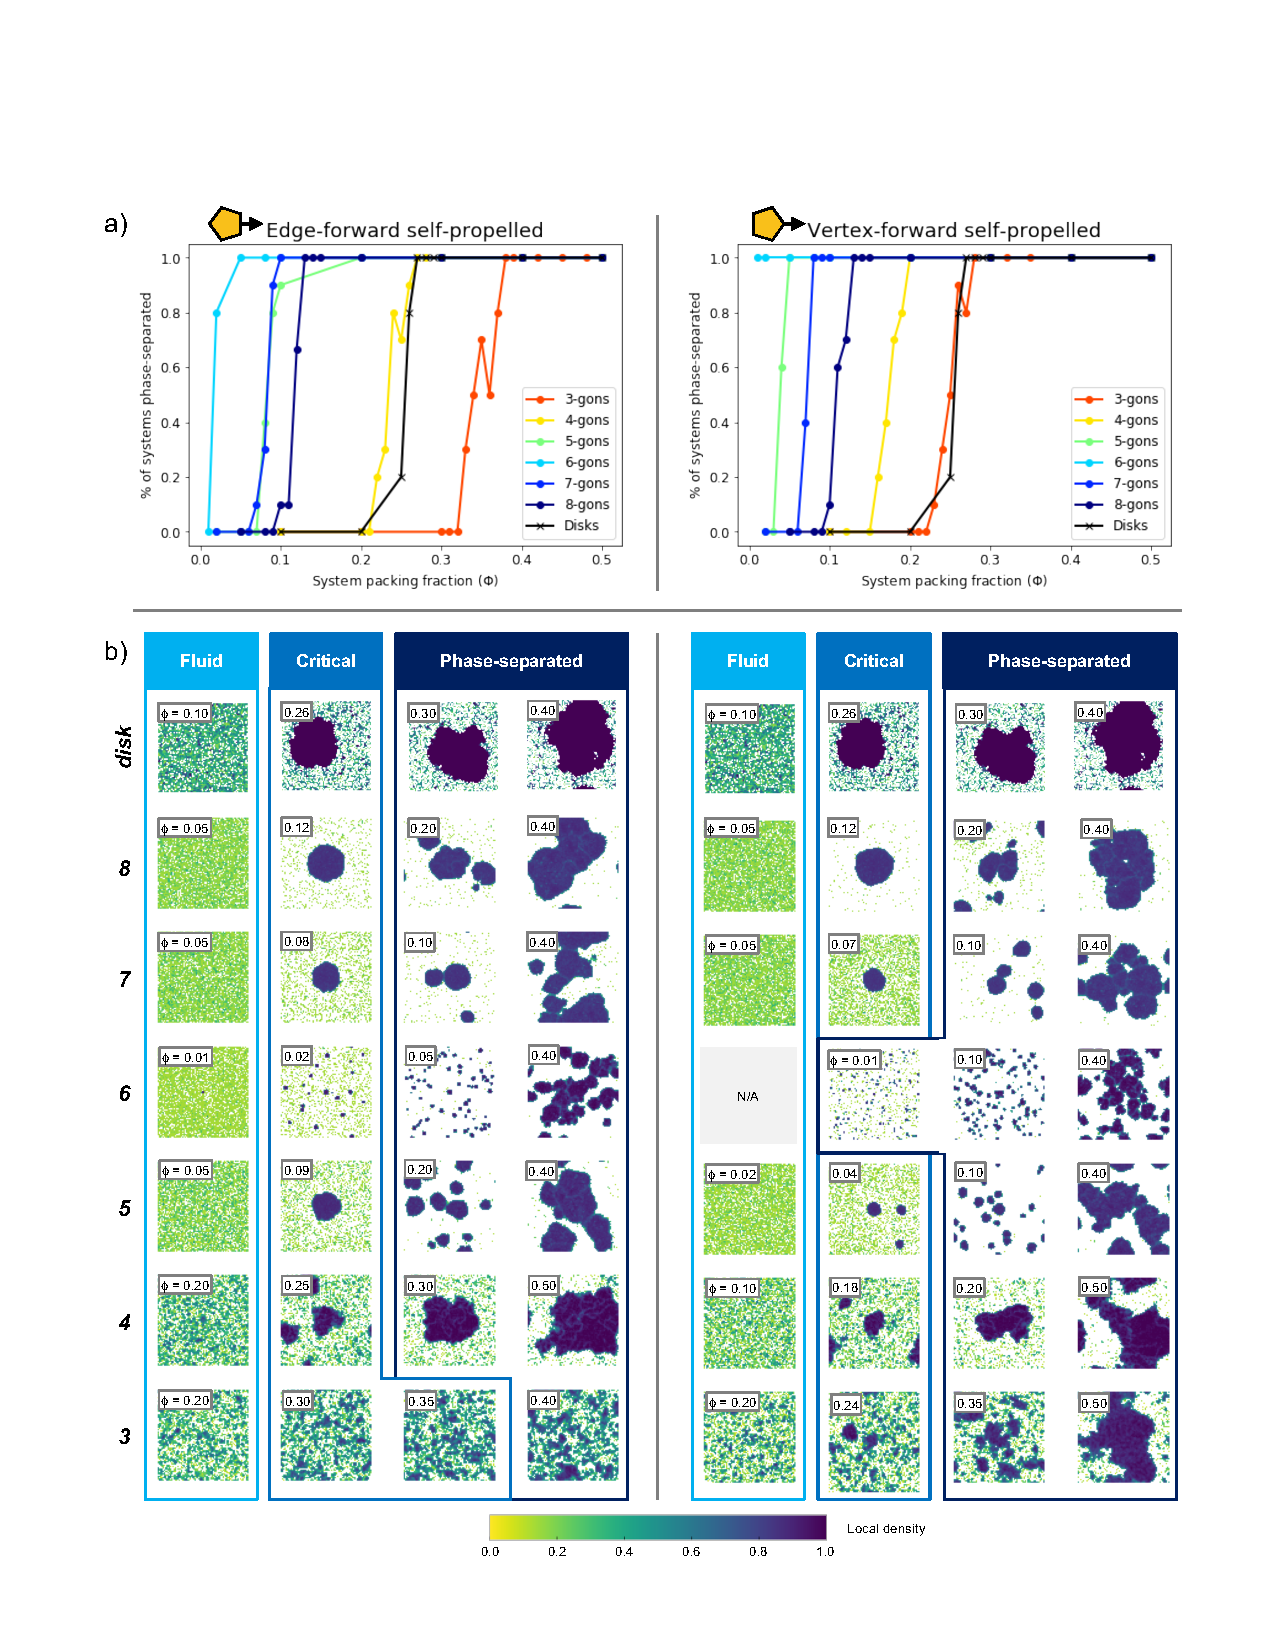
\includegraphics[width=6.5in]{../figures/Fig2.pdf}
\caption{\textbf{Critical density and nucleation behavior}: (A) Average domain size (cluster size? grain size?) versus time is different for disks versus shapes, and also depends on force director. (B) Critical density, the density at which SOME DEF OF CLUSTERING OCCURS, depends on both shape and direction of force director.}
\label{fig:phase_diagram}
\end{center}
\end{figure}

\begin{figure}[t]
\begin{center}
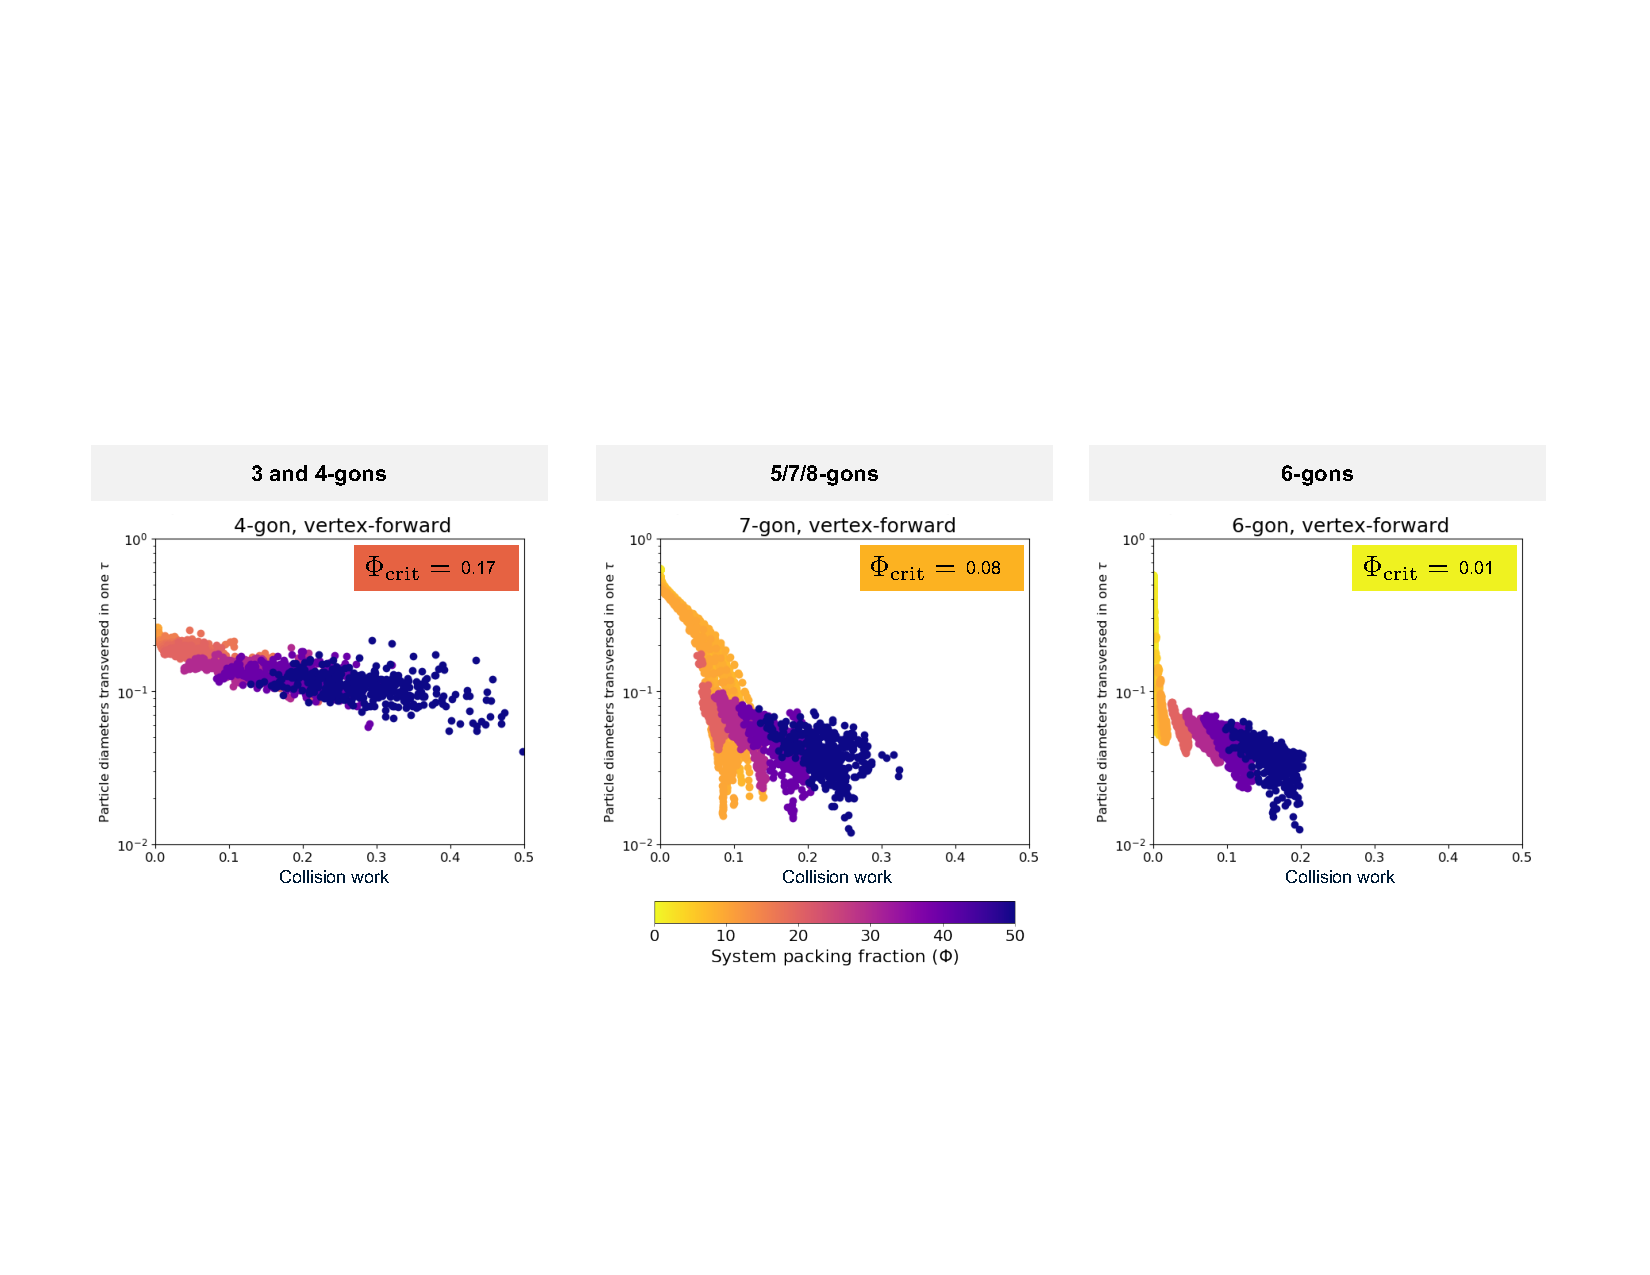
\includegraphics[width=6.5in]{../figures/Fig3.pdf}
\caption{\textbf{Collision efficiency}: Something with pressure? Not sure how to use this yet, but feel like there's something here...}
\label{fig:pressure}
\end{center}
\end{figure}


\begin{figure}[t]
\begin{center}
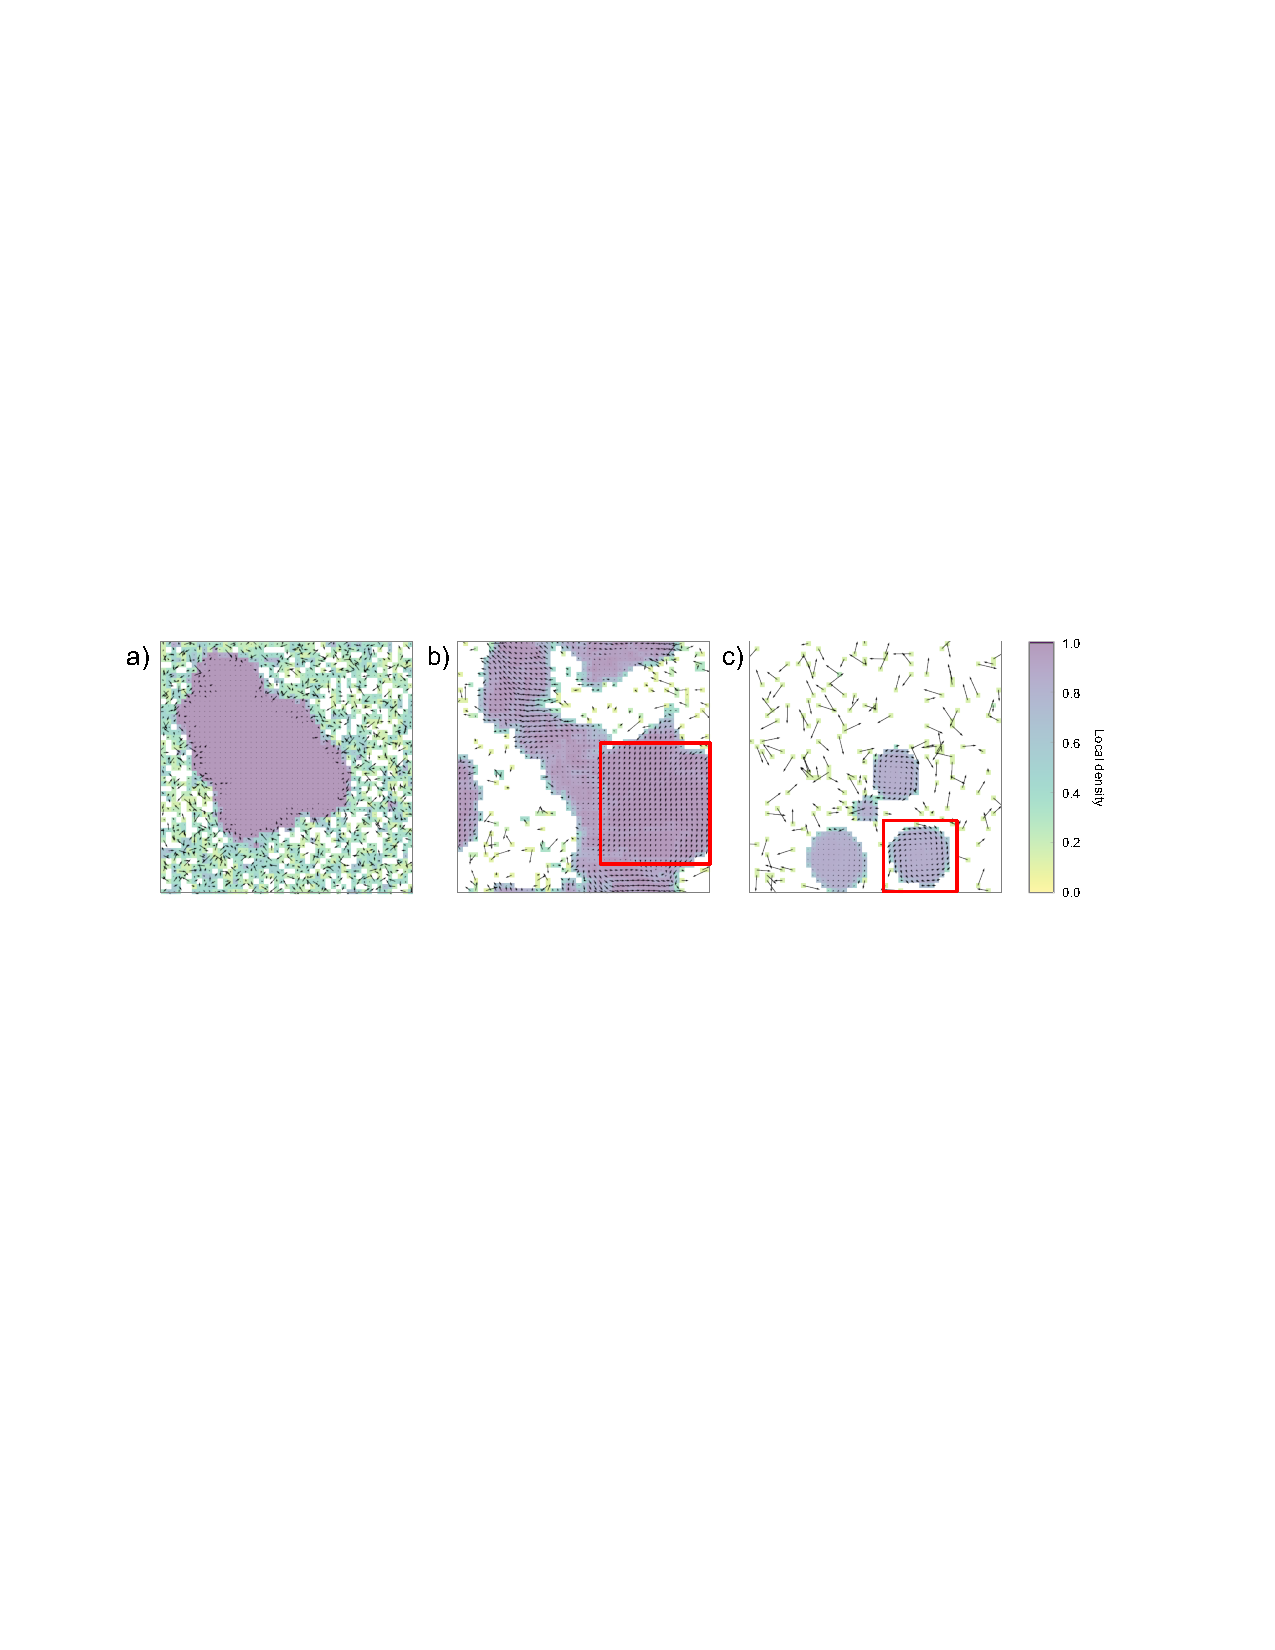
\includegraphics[width=6.5in]{../figures/Fig4.pdf}
\caption{\textbf{Displacement fields}: In contrast with disks, clusters are able to convert translational forces into rotation (highlighted in red boxes). Clusters of disks can?t sustain translational or rotational motion? clusters of shape can (this was off-hand noted in Suma et al)
}
\label{fig:velocity}
\end{center}
\end{figure}

\section{Previous work}

The research proposed above utilizes a different system from my work to date.
While the proposed research looks at the interplay of folding geometry and non-specific attractions on equilibrium assembly, I previously studied the role of hard particle shape interactions in an actively driven system. 
Consistent in this research is an interest in understanding, and characterizing, the role of particle interactions on self-assembly.
Below is excerpted from an in-preparation paper detailing the role of anisotropy on self-assembly in active systems \cite{Moran_2018_unpublished}. 

\subsubsection*{Background}

Active matter has been a field of rapidly expanding interest and research activity over the last decade \cite{Ramaswamy_2010_AnnRevConMatPhys,MarchettiEA_2013_RevModPhys,BechingerEA_2016_RevModPhys,MarchettiEA_2016_CurrentOpinionColloidInterfaceScience}.
Vicsek's pioneering work showed that collections of point particles with alignment rules displayed rich collective behavior, including phase separation \cite{VicsekEA_1995_PRL}.
However, theoretical work seeking to describe the collective behavior of bacteria demonstrated that phase separation was not reliant upon explicit alignment rules \cite{Cates_2010_PNAS}.
Giant number fluctuations characteristic of phase separation in these systems of isotropic particles were found to lead to phase separation based on density-dependent slowing in a phenomena now known as ``motility-induced phase separation'' (MIPS) \cite{CatesTailleur_2013_EPL}. 
This phase separation in isotropic systems has been described as athermal phase separation \cite{FilyMarchetti_2012_PRL}, kinetic steady-state balancing of particle fluxes \cite{RednerEA_2013_PRE, RednerEA_2013_PRL}, classical nucleation \cite{Richard_2016_SoftMatter,Redner_2016_PRL}, and balancing of collision theory timescales \cite{Bruss_2017_arxiv}.
Importantly, this same phase separation predicted by theory has been observed in experiments, which confirm the activity-dependent formation of ``active crystals'' at low system densities \cite{PalacciEA_2013_Science,PetroffEA_2015_PRL}.

However, in real-world systems (e.g. bacteria) particles are rarely isotropic.
Simulations of rods with varying aspect ratios have been shown to display a rich variety of collective motion dependent on shape and system density \cite{WensinkLoewen_2012_JPhysConMat,YangEA_2010_PRE}.
Drawing from the example of anisotropic swimmers such as bull sperm and \textit{Chlamydomonas}, Wensink \textit{et al} observed that shape and direction of the translational driving force relative to the shape (referred to as ``force offset'' in this paper) allowed for differing modes of collective motion and onset of critical behavior \cite{Wensink_2014}.
Similarly, gear shaped ``spinners'' with differing directions of a rotational driving force were shown to phase separate through competing steric interactions (repulsive for opposite spinners, and attractive for like spinners) \cite{NguyenEA_2014_PRL, SabrinaEA_2015_SoftMatter, SpellingsEA_2015_PNAS}.
In a study of active dumbbells, Suma \textit{et al} noted that particle anisotropy allowed for stabilization of cluster rotation, a phenomenon not seen in clusters of isotropic particles \cite{SumaEA_2014_EPL}.
Finally, a study of active squares uncovered an ``oscillatory'' activity/density regime in which large clusters would break up and re-form at steady state \cite{PrymidisEA_2016_SoftMatter}. 

Why is a description of the role of active particle anisotropy needed?
We can view this spontaneous ``phase separation'' and organization as a type of non-equilibrium self-assembly \cite{Mann_2009_NatureMaterials}.
It is well established that in the absence of attractive forces in equilibrium self-assembly, shape alone is sufficient to determine the minimum free-energy structure \cite{Onsager_1949_ANYAS,Damasceno_2012_Science,Manoharan_2015_Science,vanAndersEA_2014_PNAS}. 
While self-assembling, fluctuations allow a system to randomly sample system configurations until it finds the one with the minimum free energy.
However, sometimes the global free energy minimum is kinetically difficult to reach, and the system can become kinetically trapped in a metastable state.
Activity provides a driving force which can help anneal a system out of these kinetic traps \cite{VanDerMeerDijkstraFilion_2016_SoftMatter,Mallory_2016_PRE} or stabilize system configurations that would be unstable without the additional driving force \cite{ZhangYanEA_2016_AngewandteChemie}. 
Understanding how particle anisotropy combined with an active force director will impact the collective motion, even in the form of a general heuristic, would open the doors to studying non-equilibrium self-assembly tailored through particle anisotropy. 

\begin{figure}[t]
\begin{center}
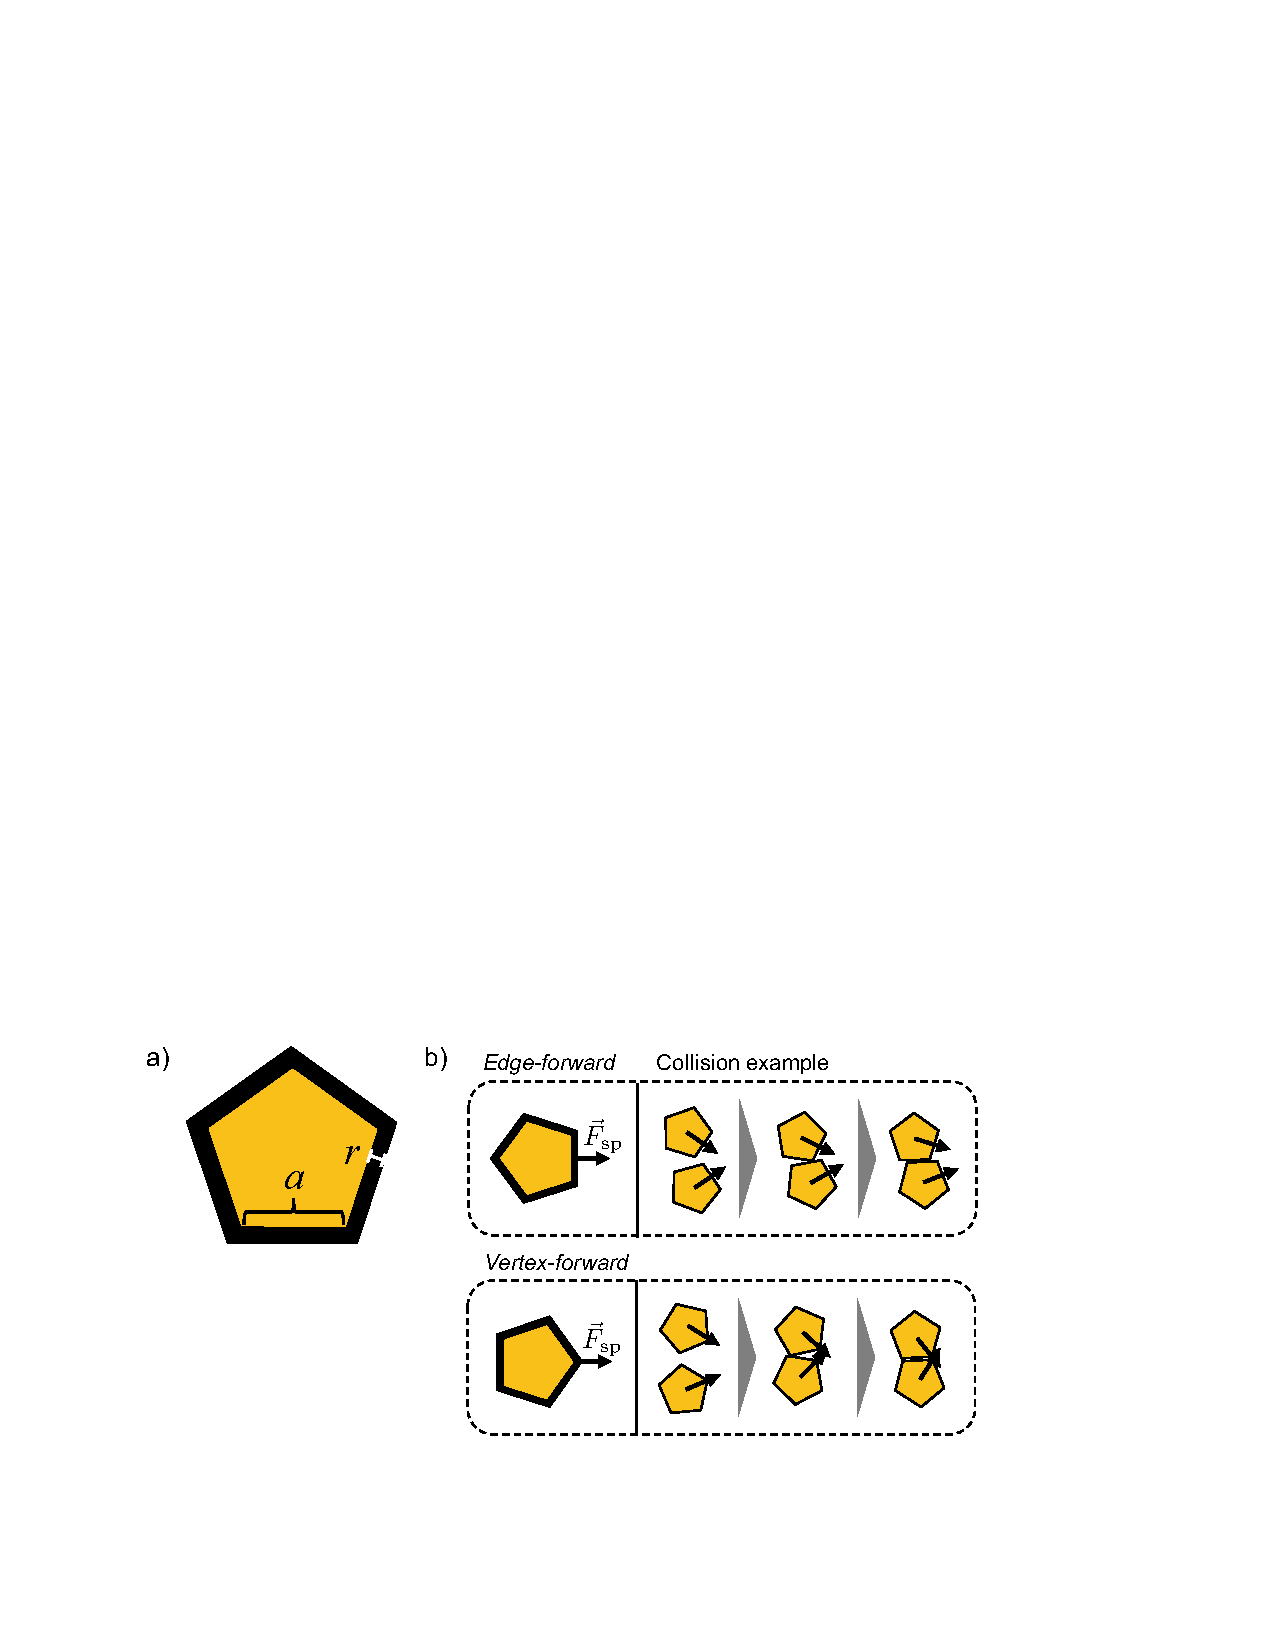
\includegraphics[width=4in]{../Figures/Fig1.pdf}
\label{fig:model}
\end{center}
\caption{
\textbf{Model system}:
(a) Shape anisotropy is studied with a family of regular polygons of side number $n=3-8$, characterized by side length $a$.
Particles interact through a purely repulsive WCA potential of radius $r=1$.
The dimensions of all shapes are set such that $\frac{n{\cdot}a}{2{\pi}r}=0.9$.
(b) Force anisotropy is implemented through the direction of the self-propelling force, which propels the shape either edge- or vertex-forward.
A key feature of this system is that collisions of anisotropic particles can sustain dimer (and larger n-mer) translational and/or rotational motion.
Illustrative collisions are provided for each force director.
}
\end{figure}

%In all studies of active shapes, some degree of particle ordering has been found in the clusters. 
To date, the differing behavior between active disks and active shapes has been explained in system-specific terms. 
Here, we study a system of active shapes to systematically understand and describe the role both shape and force anisotropy play in the collective behavior of translationally-driven active systems using the model shown in Fig. \ref{fig:model}.
Shapes are implemented using the discrete element method \cite{DEM_2017} implemented in HOOMD-blue \cite{HOOMD_2008, HOOMD_2015}.
We use Langevin dynamics to model the movement of the particles studied here, and take care to select a sufficiently small mass that the system is effectively Brownian, in line with the expected dynamics of bacteria.
Full simulation parameters can be found in the Methods section of the in-preparation paper.
\section*{Results}

% =====
% CRITICAL DENSITY
% =====

\subsection*{Critical density}

We characterize phase separation in terms of a ``critical system density'' at which the system separates into a sparse gas phase and dense clusters (based on a local density calculation detailed in the Methods section of the in-preparation paper).
We would expect that particle anisotropy should depress critical density relative to that seen in disks \cite{PrymidisEA_2016_SoftMatter}.
If we hypothesize that clustering follows the same mechanism as an equilibrium phase transition, we would expect the nature of this ``transition'' to mirror that of these shapes in equilibrium.
Specifically, work by Anderson \textit{et al.} suggested that shapes beyond 7-gons display a phase transition from fluid to hexatic to solid analogous to the transition seen in disks.
Naively, we might then expect that the critical density will decrease with decreasing $n$, and would expect phase separation behavior for $n{\geq}7$ to be indistinguishable from disks.

As shown in Figure \ref{fig:phase_diagram}A, we do observe a change in critical density relative to that seen in disks.
However, critical density does not correlate linearly with the number of particle sides, and is not uniformly depressed by the introduction of shape.
Instead, we see 6-gons phase separate at extremely low packing fractions (even at $\Phi=0.01$ in vertex-forward models). 
Next, 5-, 7-, and 8-gons phase separate at moderately low packing fractions.
Finally, 3- and 4-gons phase separate at similar or even higher critical densities than those of disks.

At first glance, this trend appears to correlate with (1) the free volume in the cluster and (2) the ability of the shape's densest packing to stabilize shear.
Particles in the cluster attempt to pack into their shape's densest packing \cite{AtkinsonEA_2012_PRE} (results not shown in Prelim Report).
For 6-gons, this results in a honeycomb lattice, while 5-, 7-, and 8-gons assemble into lattices with interstitial free space.
While 3- and 4-gons can completely tile space, their densest packings are not able to stabilize shear forces in the cluster. 
Unlike clusters of disks, which cannot sustain translational or rotational motion, clusters of shapes can maintain momentum.
This directional movement enables both stabilized grains and shear stresses between grains not seen in disks.
Consequently, clusters of 3- and 4-gon are fundamentally less stable than their higher-$n$ counter parts. 
This explanation also explains Prymidis \textit{et al}'s discovery of an ``oscillatory'' regime in their phase diagram \cite{PrymidisEA_2016_SoftMatter}.
We would expect to see such a regime in any shape whose densest packing is prone to shear planes.


\newpage
\vfill

\begin{figure*}[!ht]
\begin{center}
% width should be 17.8cm, cut to make room for caption until I can cut it down
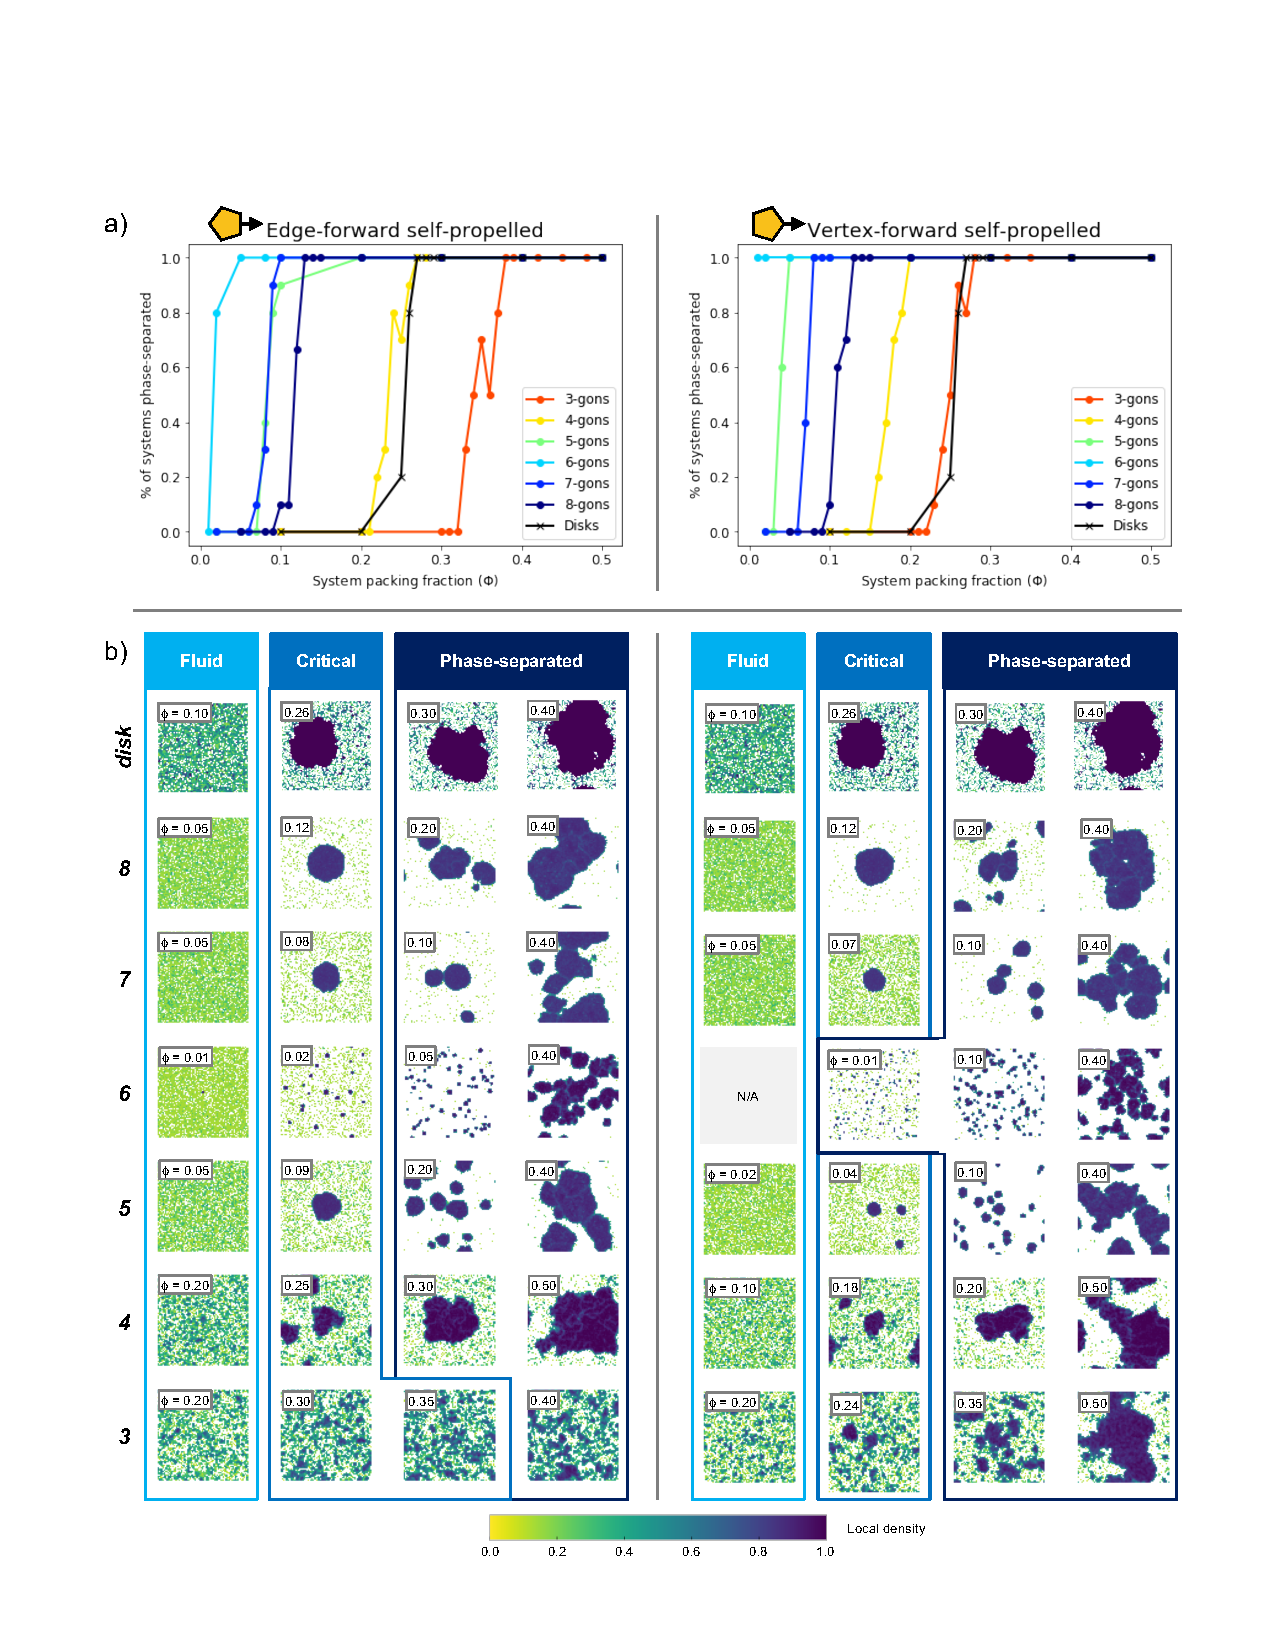
\includegraphics[width=6in]{../Figures/Fig2.pdf}
\caption{
\textbf{Critical density and nucleation behavior}:
(a) Ten replicates are studied at each $n$-gon and system packing fraction, and the fraction of replicates that phase-separate at steady state is determined as described in the Methods.
We see that the transition to phase separation is an abrupt one versus system packing fraction.
(b) Representative snapshots for the fluid (${\leq}0.10$ of systems phase separated), critical ($>0.1$ and $<0.9$), and phase-separated (${\geq}0.9$) regimes.
A distinctive feature of phase separation in systems of anisotropic particles is the formation of multiple stable clusters.
Large clusters at high packing fractions are formed by the collision of these multiple clusters.
%Grain boundaries resulting from these collisions can be seen in SI Figure \ref{sifig:structure}.
}
\label{fig:phase_diagram}
\end{center}
\end{figure*}

\vfill
\clearpage


% =====
% COLLECTIVE BEHAVIOR
% =====

\begin{figure*}[!t]
\begin{center}
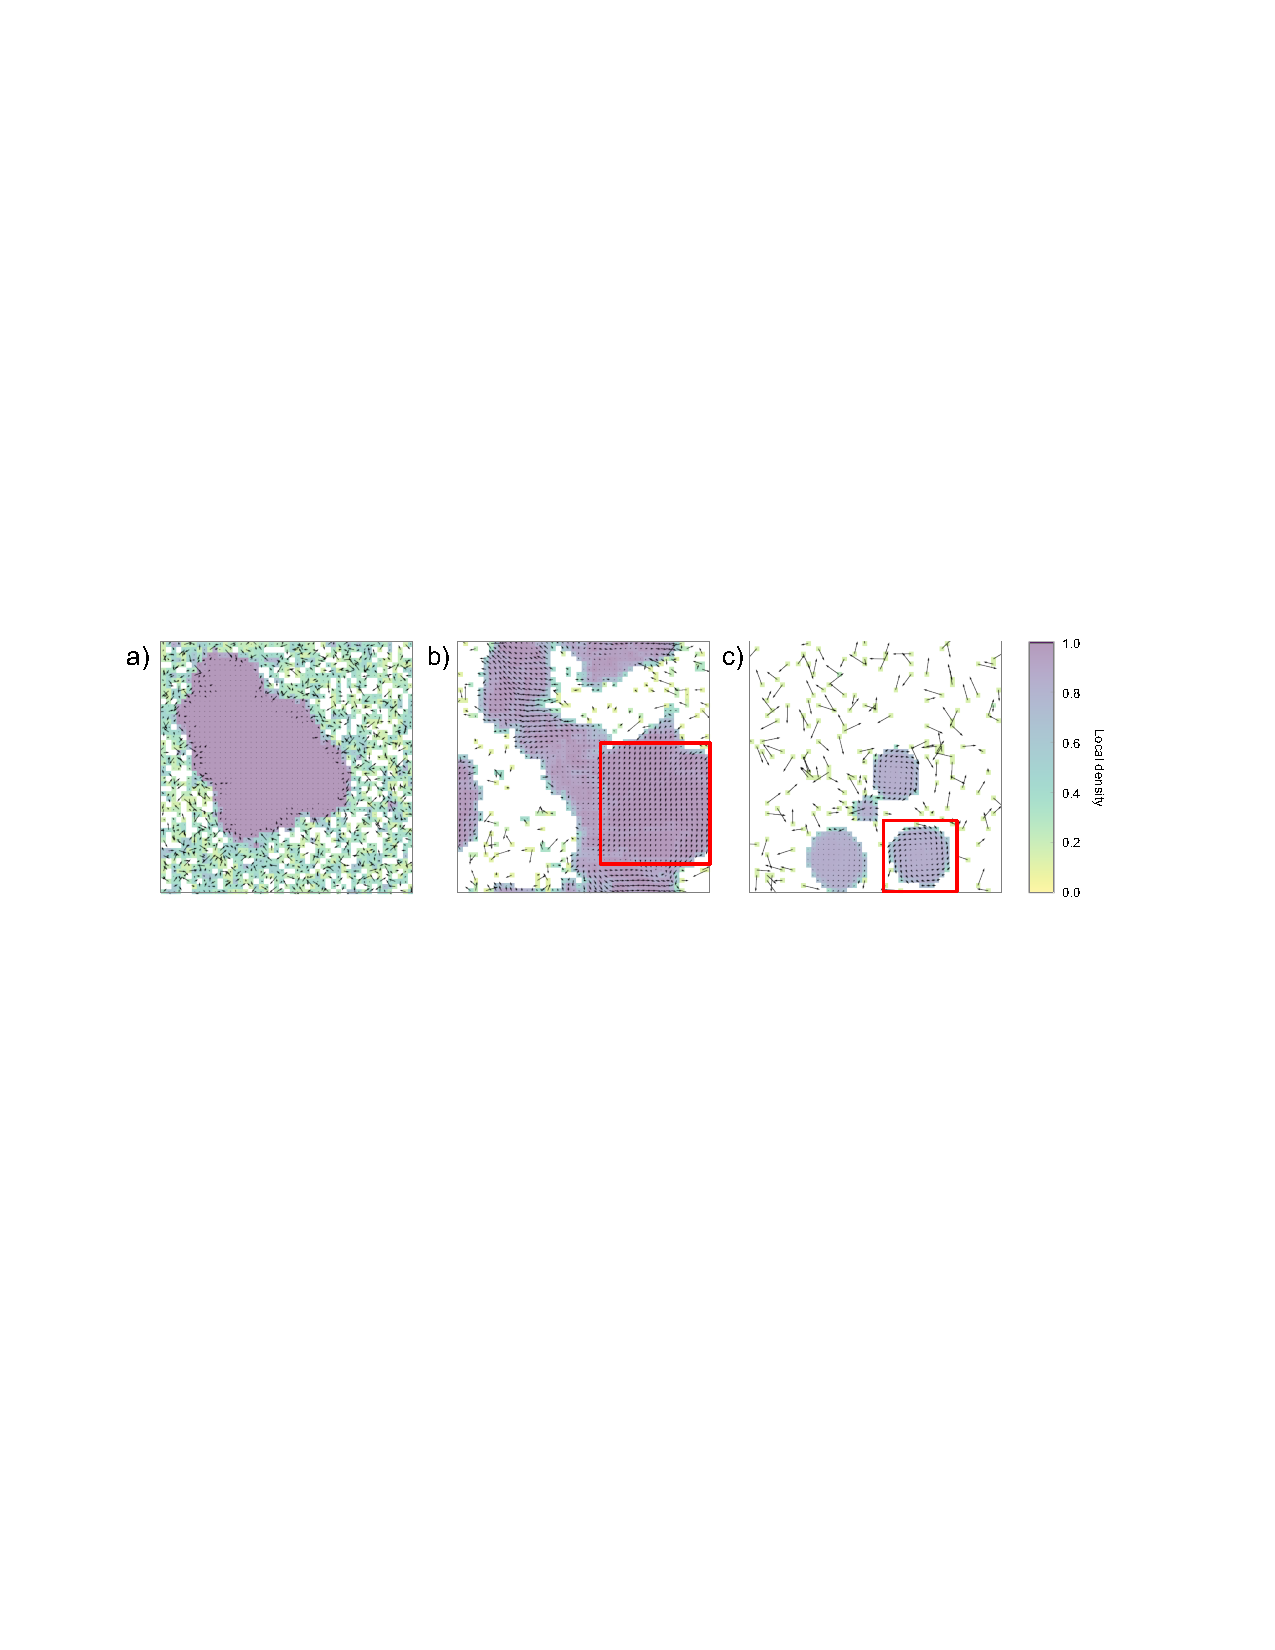
\includegraphics[width=6in]{../Figures/Fig4.pdf}
\caption{
\textbf{Cluster displacement}:
Shown are the particle displacement fields for simulations at steady state, laid over a map of local densities. 
(a) Clusters of disks have no net motion, with particle motion limited to the cluster boundaries and gas phase.
(Shown is a system of disks at $\Phi=0.3$).
In contrast, clusters with of shapes are able to convert particle translational forces to net motion (red insets).
Such clusters display both
(b) net translational motion (shown for $n=4$, $\Phi=0.5$, vertex-forward) and
(c) net rotational motion (shown for $n=7$, $\Phi=0.1$, edge-forward).
}
\label{fig:velocity}
\end{center}
\end{figure*}

\subsection*{Collective behavior}

Prior studies of driven shapes have observed that clusters are able to sustain rotational \cite{SumaEA_2014_EPL} and translational motion.
We also observe this behavior, as seen in Figure \ref{fig:velocity}.
As shown in Fig \ref{fig:velocity}A, clusters of disks do not have rotational or translational motion.
The only net motion within the cluster is at the boundaries, where a balance of particle fluxes in/out characterize the steady state configuration \cite{RednerEA_2013_PRL}.

However, to the best of our knowledge, other studies have not observed a key consequence of this ability: the formation of multiple small, stable clusters as precursors to bulk phase separation.
As seen in Fig. \ref{fig:phase_diagram}, phase separation in 5-, 7-, and 8-gons is characterized by the formation of one or few clusters which nucleate and grow.
In 6-gons, cluster nucleation is so favorable that we see the nucleation of many small clusters even in the critical regime.
For 3- and 4-gons, this picture is less clear but still points towards the formation of multiple small clusters as pre-cursors to phase separation.

In viewing videos of the evolutions of these systems (available during Preliminary Oral Exam), we see that at intermediate densities, these small clusters are stable.
This can also be seen in Figure \ref{fig:velocity}C, in which clusters are spinning in place.
At higher densities in systems of shapes, multiple small clusters form and translationally collide with one another to create larger clusters; evidence of these collisions can be seen in grain boundaries in large clusters at steady state.

In contrast, systems of isotropic particles cannot have multiple clusters collide, as clusters cannot sustain the motion required for a collision.
Instead, while multiple clusters may nucleate, a final system cluster is caused by either (1) smaller clusters dissolving and one large cluster dominating or (2) multiple smaller clusters merging into one another as they grow.
A steady state of multiple small clusters would be highly unlikely in a system of isotropic particles, as clusters in such systems are only stabilized by particles being self-propelled into the cluster.

This suggests that particle anisotropy allows these systems to pursue a different mechanism of nucleation.
Importantly, this mechanism of cluster formation does not appear to be achievable in disks. 
Redner \textit{et al.} investigated the addition of attraction to active isotropic particles at a constant packing fraction of $\Phi=0.4$ \cite{RednerEA_2013_PRE}.
At high activity and low attraction, that study replicated the formation of one large cluster seen in the literature.
At lower activities and high attraction, they were able to access a gel state; however, at no point in the activity/attraction phase space were multiple, clearly-separated stable clusters observed.  

% =====
% IMPACT OF SHAPE
% =====

\begin{figure*}[!t]
\begin{center}
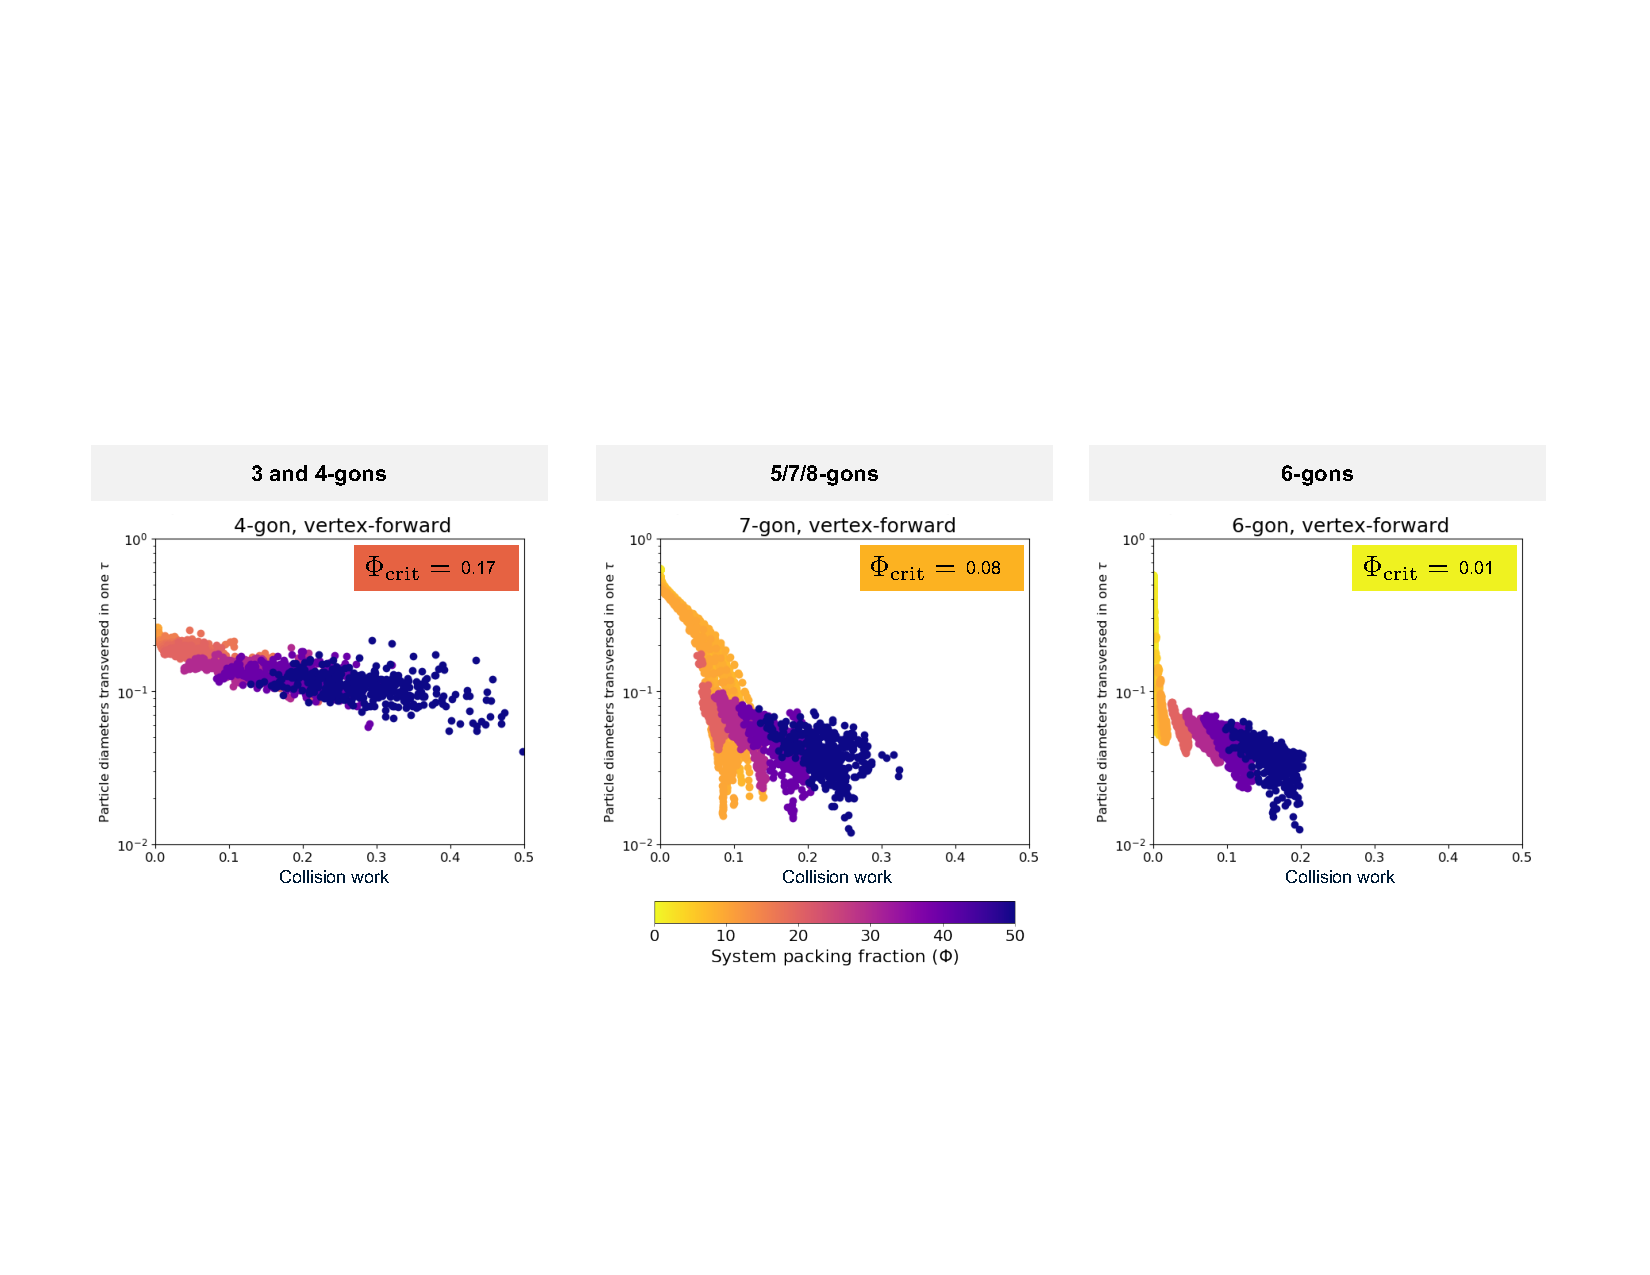
\includegraphics[width=6.5in]{../Figures/Fig3.pdf}
\caption{
\textbf{Collision efficiency}:
Shown are the evolution of particle velocity versus work done by inter-particle collisions in a system over the course of simulation.
Each system packing fraction is composed of ten replicates, with data snapshots taken approximately every $125\tau$.
Statepoints shown are representative of behavior in each group of $n$-gons.
}
\label{fig:pressure}
\end{center}
\end{figure*}

\subsection*{How anisotropy impacts the collective behavior}

While it is clear that shape and force anisotropy work together to impact the critical density and nucleation behavior, an explanation from existing theories is less clear. 
A kinetics-based theory developed in \cite{Redner_2016_PRL} treats cluster formation as a balance of in/out fluxes of particles at the boundary of a cluster.
This balance relies upon the assumption that particles can escape clusters when the direction of their active force diffuses above the horizon of the cluster (either solo or as part of a multi-particle escape event).
However, such diffusion is significantly stericly hindered in clusters of shapes.
While these assumptions work well in systems of disks where they correctly predict the formation of a large cluster which nucleates and grows in cases of phase separation, it is not clear how to tailor this theory to the behavior of systems of anisotropic particles. 

Alternatively, we can take a collision-theory based approach as described in \cite{Bruss_2017_arxiv}, which treats phase separation as the result when the average collision time ($\tau_C$) exceeds that of the average particle's free time between collisions ($\tau_F$).
Calculating the $\tau_F$ of the particles and assuming a constant $\tau_C$ for all shapes, we would expect to find 3-gons with the lowest critical density, with 8-gons the highest, not in line with our simulation results.
This confirms our intuition that the mechanism by which shapes depress the critical density is by increasing the collision time.

We posit that this increased collision time is the result of ``more effective'' collisions between some shapes versus others.
In the context of MIPS, we can  say that ``more effective'' collisions are those that translate inter-particle forces-- collisions-- to greater decreases in particle velocity.
That is, for a given collision, collisions between some particle shapes will lead to a steeper decreases in particle velocity than others.  
This also re-affirms our decision to study emergent behavior versus system density, a good proxy for the likelihood of inter-particle collisions that are required for phase separation to occur.

We can measure the net work done by all inter-particle collisions in the system as $ W = \frac{1}{2}\sum_i\sum_{j{\neq}i} \vec{F_{ij}}{\cdot}\vec{r_{ij}} $, where where $\vec{F_{ij}}$ and $\vec{r_{ij}}$ are the pairwise forces and distance between particles, respectively.
To study the efficiency of collisions for different shapes, we plot velocity versus the system's ``collision work'' in Figure \ref{fig:pressure}.
The velocity is shown as a percentage of the terminal velocity a particle would reach if it experienced no collisions.

We see that the evolution of velocity versus work done by collision follows very different patterns for the three groups of shapes.
Velocity quickly decreases with very little work for 6-gons, while velocities of 3 and 4-gon systems change little with collisions.
As might be expected from earlier results, 5/7/8-gons fall somewhere in between.

As presented, this data shows the time evolution for systems at each density, from start of the simulation (higher velocity) through steady state (lower velocity).
Next steps will be to probe the relaxation time from this data, which we expect to be shape-dependent given the obvious difference in velocity/work relationships in the critical regime for each group of shapes.
We are hopeful this will provide a definitive explanation for the role of shape in these systems.

%Enhanced collision time due to particle anisotropy allows such particles to phase separate at lower critical system densities than isotropic particles.
%We can borrow some concepts from percolation theory to think about this.
%Instead of the probability of a site being occupied, we have the probability of a collision (per some unit time) occurring at a given system density.
%The fraction of systems that phase-separated at a given system density, then, are analogous to the probability of there being a percolating cluster in a given sample



%\section*{Discussion and conclusions}

While the nature of the densest packing in equilibrium can be used to explain the collective behavior seen under activity, further work is needed to elucidate the link between equilibrium packing (or assembly) and non-equilibrium assembly.

Finally, one may argue that the clusters observed here are kinetic packings, rather than thermodynamic self-assembled states.
As the thermodynamics of active matter continues to develop, establishing the phase behavior of active assemblies (or packings) will be of intense interest as directed, non-equilibrium self-assembly is developed.
%% =====
% Model and dynamics
% =====
\subsection*{Model and dynamics}

We study a family of regular polygons of side number $n=3-8$, shown in Fig. \ref{fig:model}A.
Polygons are modeled as hard particles that interact via a purely repulsive contact potential.
This contact is modeled with a Weeks-Chandler-Anderson (WCA) potential of radius $r=1$ \cite{WCA_1971}.
We set particle side length $a$ to maintain a constant $\frac{\sum_is_i}{2\pi r}=9$ for $r=1$.

We also explore anisotropy in the direction a constant active force ($\vec{F}_A$) applied to each particle.
We set $\vec{F}_A$ to be either perpendicular to a side of the particle (\textit{edge-forward}) or directed directly out a corner (\textit{vertex-forward}), with the orientation of the director locked to the particle.
Rotational noise of the particles allows the active force to diffuse with particle rotation. % implemented through the integrator

All simulations are run with $\Pe=150$, where $\Pe$ is a measure of active (advective) to diffusive motion. \textcolor{red}{Add formula for \Pe here.}
In this regime, thermal fluctuations contribute much less to the motion of the particles than does the active driving force.
To keep the $\Pe$ value constant across all simulations, the magnitude of the active force ($|\vec{F}_A|$) set to 1 and the temperature of the thermal bath governing the fluctuations is set as $T = \frac{|\vec{F}_A|*\sigma}{\Pe}$.

Particle motion is solved for using Langevin equations of motion.
The magnitude of rotational and translational noise is implemented in the integrator as a function of $T$.
The magnitude of the random force ($\vec{F}_R$) is chosen via the fluctuation-dissipation theorem to be consistent with the specified drag and temperature, $T$.
To closely approximate Brownian motion, mass of the particles is set to $m=1e-2$.

The Langevin equations of motion with an active driving force are given by:
$$ m\frac{\d\vec{v}}{\d t} = \vec{F}_C - \gamma\cdot\vec{v} + \vec{F}_R + \vec{F}_A $$
$$ \langle |\vec{F}_R|^2\rangle = 2dkT\gamma/\delta t$$

Here, $\vec{F}_C$ is the force on the particle from all potentials and constraint forces, $\gamma$ is the drag coefficient, $\vec{v}$ is the particle's velocity, and $d$ is the dimensionality of the system (2). 
We approximate the rotational friction drag coefficient in 2D, $\gamma_r$, as a function of the translational friction coefficient $\gamma$ per the Stokes-Einstein relationship: $\gamma_r = \frac{\sigma^2\gamma}{3}$.
We set the translational drag coefficient $\gamma$ to 1 and calculate $\sigma$ as the diameter of an equi-area disk to a given n-gon.


% =====
% Simulation details
% =====
\subsection*{Simulation details}

Each simulation is composed of $N=1e4$ particles, with 10 replicates run at each statepoint.
Particle positions are randomly initialized and allowed to relax with a spring potential at $\phi=0.10$ \cite{DPD_2011}.
The spring potential is then turned off and the WCA pair potential turned on (i.e. shape excluded volume) while the box compresses to the target system density.
Only after these initialization steps is the active force is turned on.
The direction of the active force is initialized randomly from the set of orientations of interest (either \textit{edge-} or \textit{vertex-facing}).

The simulation is run for $5000\tau$ with a timestep of $dt=1e-3$ (where $\tau = \frac{\sigma\gamma}{|\vec{F}_A|}$, the time it takes a particle to actively travel its own particle length).
We validate that simulations have reached steady state by the end of these simulations by validating that the system pressure has reached steady state (see SI Fig \ref{fig:SSpressures}).
\textcolor{red}{Check against this paper in case there are any claims I should be aware of: \cite{SolonEA_2015_NaturePhysics}.}
The system is initialized for $5e5$ time steps, and compressed to the target density for $5e5$ time steps.

Langevin dynamics simulations are performed on graphic processing units (GPUs) with the HOOMD-blue software package \cite{HOOMD_2008, HOOMD_2015}.
Shape interactions are modeled using the discrete element method implemented in HOOMD-blue \cite{DEM_2017}.

%TBD: How we determined the drag coefficients, rotational diffusivity to use \\
%\cite{BetEA_2016_arxiv}: Efficient shapes for microswimmers \\
%\cite{Purcell_1977_AmericanJPhys}: Life at low reynolds numbers \\


% =====
% Determining critical density
% =====
\subsection*{Determining critical density}

% Add critical density to methods, and why others from the literature can't work

There is not yet an accepted best-practice method for determining whether a system of active particles has clustered.
In one study, a system was considered ``clustered'' if the fraction of system particles in the largest cluster was ${\geq}0.2$.
However, this method is ill-suited for our systems, which include clearly phase-separated systems of many small clusters.
Next, other studies have used a local-density histogram of randomly-sampled points of the simulation box \cite{Bruss_2017_arxiv}.
If the histogram displayed two peaks, the system was considered phase-separated.
However, the very low system densities studied here limit the efficacy of this approach (i.e. at a packing fraction of 0.01, the high-density ``peak'' would be ${\leq}2\%$ the magnitude of the larger peak).

To determine phase separation even at low densities, we calculate two separate histograms of local densities at a radius of \textcolor{red}{X} from : (1) randomly sampled points ($N=1e5$) and (2) about each particle ($N=1e4$).
We then calculated a position-normalized local density histogram of the system by multiplying the frequencies of local densities in each bin by one another.
If the resulting histogram has a high-density peak ${\geq}20\%$ the height of the low-density peak, we consider the system to be phase-separated.

The fraction of systems that has phase-separated for a given system packing fraction is the fraction of the ten replicates run at each packing fraction which has phase separated, based on the above criteria.








\section{Conclusions and potential impact}

The proposed research seeks to fill a gap in the self-assembly literature: what is the minimal amount of instruction we need to give a system for it to assemble a target structure?
Recent work has shown that the interaction specificity seen in DNA-mediated addressable assembly is not specific to DNA systems \cite{Reinhardt_2014_PRL}, and that synthetic systems can replicate interaction specificity achieved by nature \cite{Huntley_2016_PNAS}.
While addressable assembly from a synthetic DNA analog has not been shown yet, an experimental realization is not far along the research horizon.
However, a core question that will need to be answered is: how much instruction will this system need to provide to successfully assemble its target structure?

The work in this PhD research proposal seeks to provide an approach and metric to answer that question. See Figure \ref{fig:gantt} for key tasks and milestones.

%Ultimately, tailoring self-assembly and addressable complexity are driven by the question:
%
%\begin{center}How do I give particles in my system sufficient information to find their proper position in a target whole?\end{center}
%
%In systems targeting particular structures, tailored attraction (experimentally via single-stranded DNA or theoretically via an attractive potential) and repulsion can be used to tailor the structure of particle assembly.
%In systems targeting addressable complexity with DNA origami and protein folding, such instruction can be given with exact detail through genetic code.
%Work by Brenner and Manoharan has sought to quantify the amount of specificity bonds in such systems can contain, and the limits on target system complexity given differing bond informations.
%
%However, missing in this conversation is a measure of the importance of each individual interaction on the emergent behavior of the whole system.
%I intend to contribute in part during the remainder of my PhD.
%Instead of simply observing emergent behavior as an outcome of specifically-designed behavior of individuals, we could instead engineer such behavior as a quantifiable outcome of the interaction of an information-rich network of agents.
%Having such knowledge may allow us to embed multiple ``states'' in a material, such as the minimum folds to move between two target origami structures \cite{An_2011_Robotica}.
%Being able to measure, and ultimately control, the assembly instructions stored in a starting material is a critical step to enabling materials by design and advancing materials science.


\begin{figure}[h!]
\begin{center}
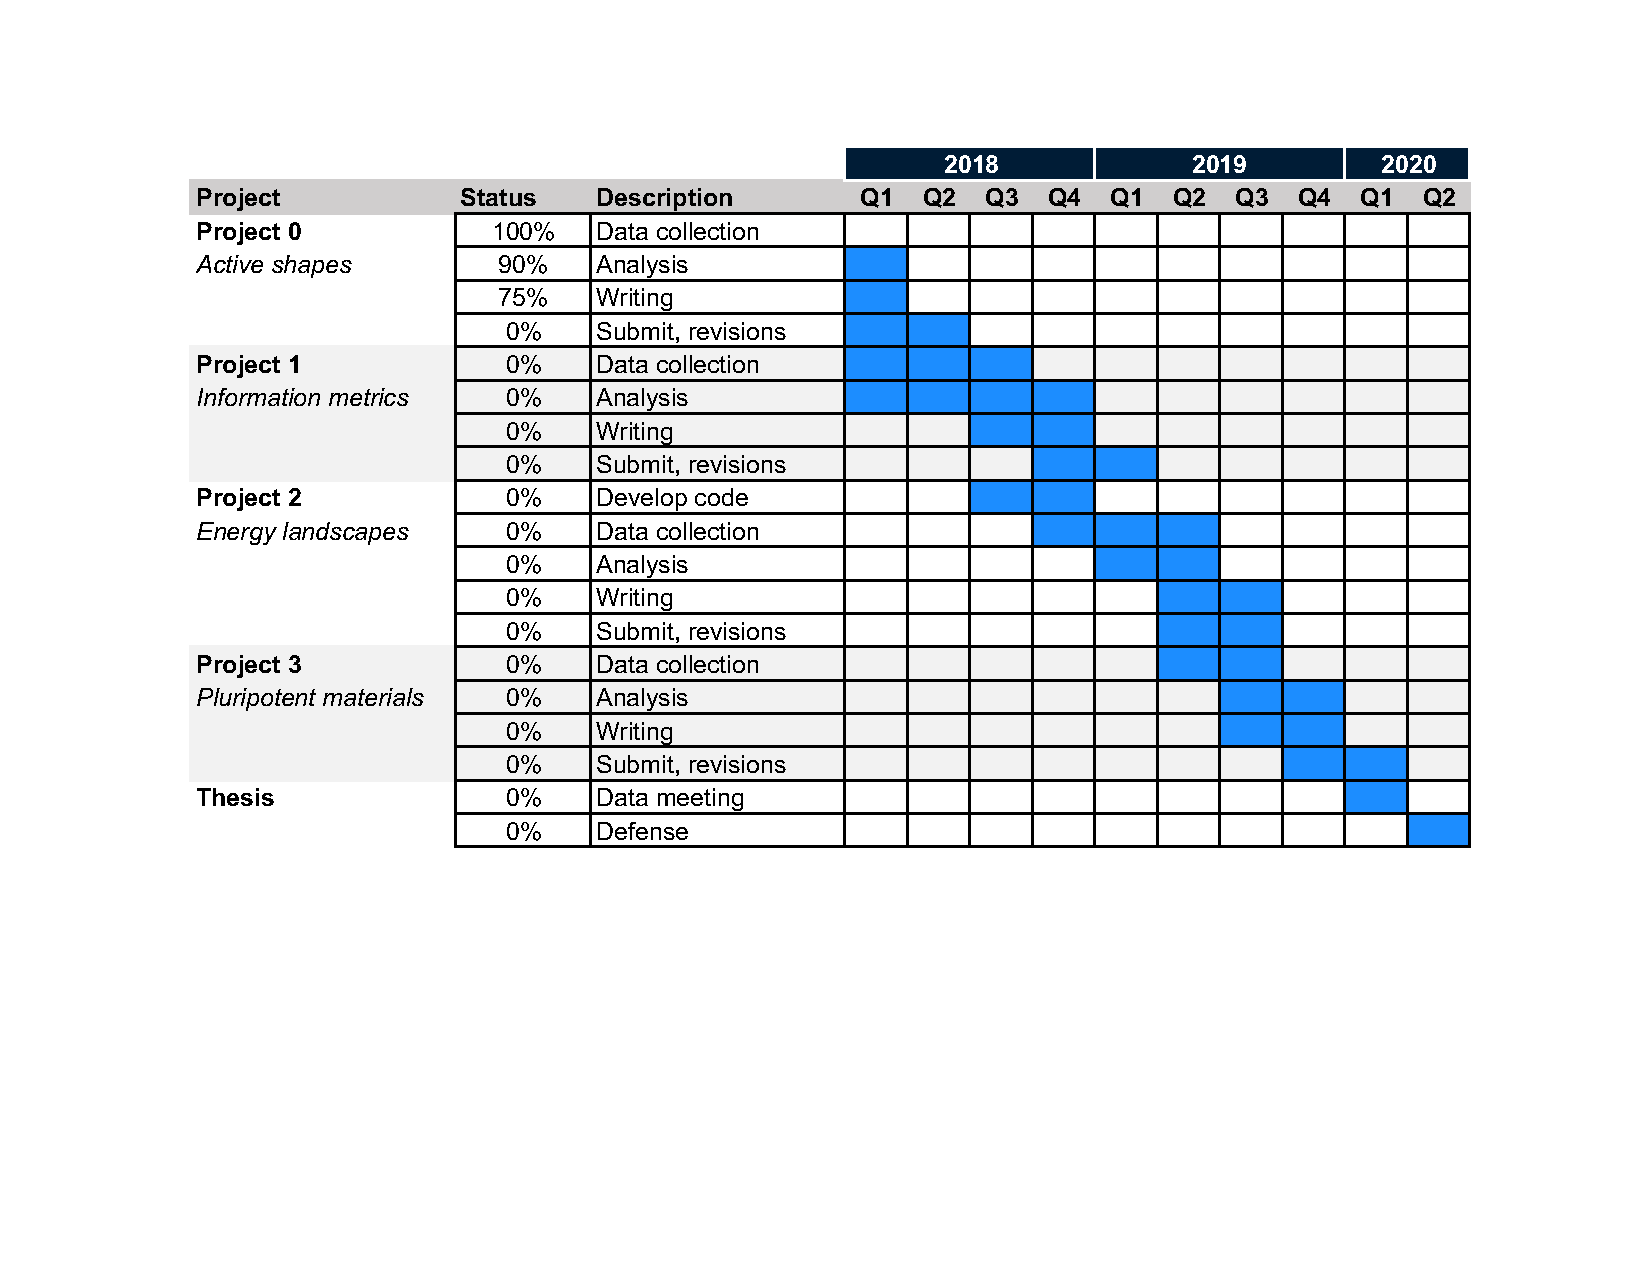
\includegraphics[height=3in]{../figures/gantt.pdf}
\caption{\textbf{Timeline}: Key milestones and tasks from Preliminary Exam through target defense date.}
\label{fig:gantt}
\end{center}
\end{figure}

% ======
% BIBLIOGRAPHY
% ======
\newpage
\bibliographystyle{unsrt}
\bibliography{../../library/_PrelimBibliography}

\end{document}